\documentclass[manuscript,screen]{acmart}
\setcopyright{none}
\acmConference[]{}{}{}
\acmYear{2026}
\acmISBN{}
\acmDOI{}

\usepackage{graphicx}

\title{Relatório Final: Análise de Desempenho de RAG Multilíngue}
\author{Luccas da Silva Lima}
\affiliation{%
  \institution{Universidade Federal do Rio Grande do Sul}
  \country{Brasil}
}
\email{luccas.lima@ufrgs.br}

\begin{document}

\begin{abstract}
Este relatório descreve a avaliação exaustiva de desempenho de um sistema de \textit{Retrieval-Augmented Generation} (RAG) em um cenário multilíngue. O experimento conduziu uma análise fatorial completa (\textit{Full Factorial Design}) para comparar a latência de geração de embeddings, a eficiência computacional (CPU, RAM e VRAM), o consumo de armazenamento e a precisão da recuperação de documentos através de 20 idiomas distintos. Utilizando um conjunto estático de documentos traduzidos por um modelo de linguagem de grande escala (LLM).
\end{abstract}

\maketitle

\section{Introdução}
A implementação de arquiteturas RAG em ambientes globais impõe desafios significativos relacionados à representação semântica interlinguística. O mapeamento de idiomas morfologicamente diversos para um espaço vetorial contínuo e compartilhado frequentemente revela disparidades de desempenho.

Considerando que a base de conhecimento permanece factualmente equivalente em todas as suas versões linguísticas, o objetivo principal desta pesquisa é isolar o impacto exclusivo do idioma nas seguintes dimensões do pipeline:
\begin{enumerate}
    \item \textbf{Custo Computacional:} Latência na codificação (\textit{encoding}) e consumo de memória ao longo da geração de embeddings.
    \item \textbf{Eficiência de Armazenamento:} Impacto da dimensionalidade e do tipo de dado (precisão de ponto flutuante) no tamanho do índice vetorial.
    \item \textbf{Qualidade de Recuperação:} Eficácia da busca por similaridade quando confrontada com nuances de tokenização e densidade informacional de cada idioma.
\end{enumerate}

\section{Metodologia e Arquitetura do Experimento}

\subsection{Reprodutibilidade}

Para garantir a rastreabilidade e a total reprodutibilidade dos experimentos, adotou-se um fluxo estruturado de desenvolvimento e gestão de dependências. Os scripts do projeto foram integralmente codificados na linguagem Python, utilizando a plataforma GitHub para o controle de versão. O repositório conta com arquivos \texttt{README} detalhados, que especificam minuciosamente o escopo do projeto e a ordem sequencial exata necessária para a execução dos códigos. Adicionalmente, a ferramenta \texttt{Poetry} foi empregada para a gerência de dependências e isolamento do ambiente virtual, assegurando a consistência das bibliotecas utilizadas e permitindo que o ambiente seja replicado fielmente.

\subsection{Ambiente de Execução}

Com exceção do processo de tradução de arquivos, o pipeline de execução foi processado inteiramente em ambiente local. As especificações técnicas da infraestrutura de hardware utilizada para rodar os experimentos estão detalhadas na Tabela~\ref{tab:ambiente_hardware}.

\begin{table}[htbp]
\centering
\caption{Especificações da infraestrutura de hardware local.}
\label{tab:ambiente_hardware}
\begin{tabular}{ll}
\hline
\textbf{Componente} & \textbf{Especificação} \\ \hline
Processador (CPU)   & Intel Core i5-12400F \\
Placa de Vídeo (GPU) & NVIDIA GeForce RTX 4060 (8 GB VRAM) \\
Memória RAM         & 32 GB \\
Armazenamento       & SSD Kingston NVMe 1 TB \\ \hline
\end{tabular}
\end{table}

A única etapa que demandou processamento externo ao ecossistema local foi a tradução dos arquivos textuais. Devido às elevadas exigências computacionais do modelo de grande porte selecionado para essa tarefa, cuja carga de trabalho excedia a capacidade da infraestrutura local disponível, optou-se pela execução desse pipeline específico por meio de requisições à API da OpenAI.

\subsection{Criação dos Documentos Originais e Tradução}
Para assegurar a paridade estrutural e semântica entre os idiomas, o corpus original foi composto por 10 documentos de referência escritos em Inglês (\texttt{en\_us}), formatados em Markdown. A expansão linguística foi conduzida através de um motor de tradução assistida por LLM (\texttt{gpt-5.1}) operando em modo \textit{zero-shot} com restrições severas (\textit{hard constraints}). O prompt garantia a preservação da formatação, impedindo sumarizações ou perda de numeração de linhas.

Esse processo, no entanto, expõe a variabilidade inerente aos idiomas. A Figura \ref{fig:char_dispersion} ilustra a distribuição de caracteres por idioma após a tradução. Nota-se que idiomas mais verbosos ou com estruturas gramaticais expansivas resultaram em contagens máximas de caracteres significativamente superiores ao original em inglês, alterando o volume bruto de dados ingeridos pelo pipeline.

\begin{figure}[htbp]
    \centering
    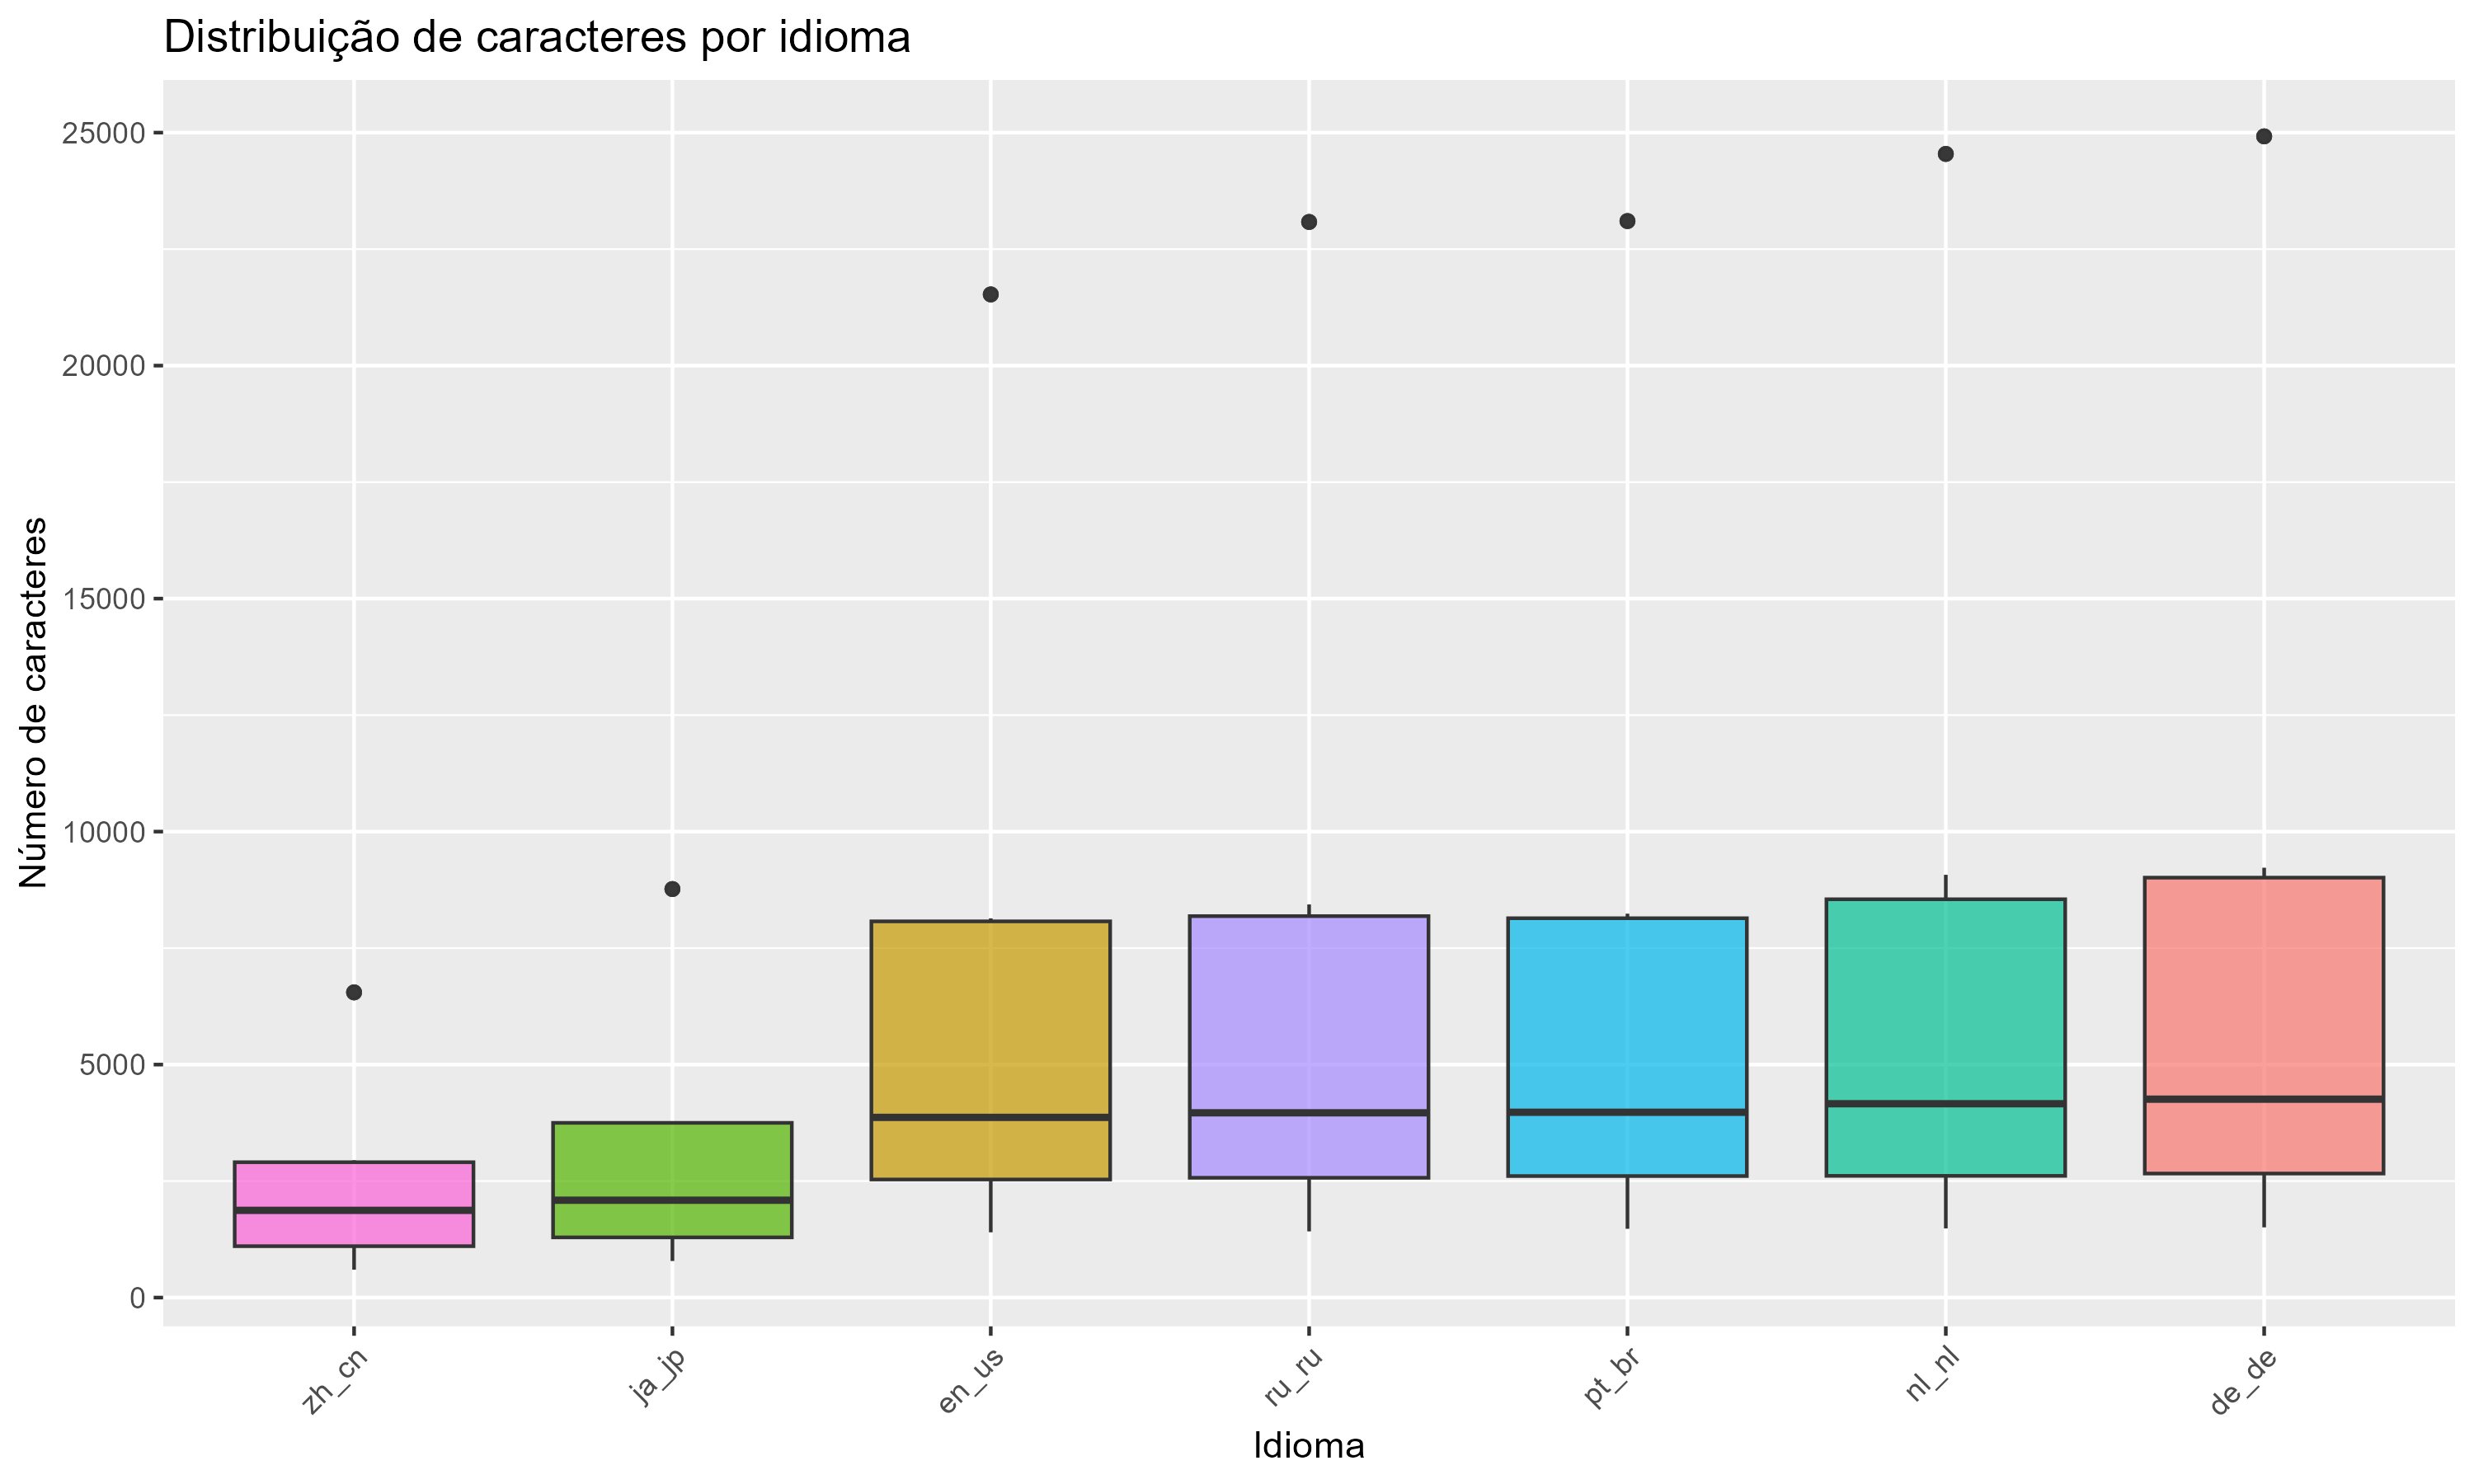
\includegraphics[width=0.8\linewidth]{../../src/results/graphs/g1_character_dispersion.png}
    \caption{Distribuição e dispersão da contagem de caracteres dos documentos traduzidos, separados por idioma.}
    \label{fig:char_dispersion}
\end{figure}

\subsection{Design de Experimentos (DoE)}

A exploração do hiper-espaço de configuração adotou um modelo Fatorial Completo (\textit{Full Factorial}), expandido para um escopo multilíngue que engloba 20 idiomas distintos. As variáveis controladas, seus respectivos níveis de variação e a volumetria total de execuções para a composição da matriz estatística estão sintetizados na Tabela~\ref{tab:doe_matriz}.

\begin{table}[htbp]
\centering
\caption{Configuração da matriz de Design de Experimentos (DoE).}
\begin{tabular}{lll}
\hline
\textbf{Fator / Variável Controlada}       & \textbf{Níveis} & \textbf{Especificação / Valores} \\ \hline
Tamanho do Lote (\textit{Batch Size})       & 7               & 7 configurações distintas \\
Tamanho do Fragmento (\textit{Chunk Size})   & 7               & 7 configurações distintas \\
Precisão Numérica (\textit{Precision})      & 2               & \texttt{float32} e \texttt{float16} \\
Métrica de Distância (FAISS)               & 2               & L2 e \textit{Inner Product} \\ \hline
\textbf{Total de Experimentos Únicos}      & \textbf{196}    & Combinação dos fatores ($7 \times 7 \times 2 \times 2$) \\
\textbf{Idiomas Avaliados}                 & \textbf{20}     & Cobertura multilíngue do estudo \\
\textbf{Replicações por Experimento}       & \textbf{10}     & Para mitigação de ruídos operacionais \\
\textbf{Total Geral de Execuções}          & \textbf{39.200} & Rodadas independentes ($196 \times 20 \times 10$) \\ \hline
\end{tabular}
\label{tab:doe_matriz}
\end{table}

Essa modelagem estruturada resulta em um montante robusto de dados, totalizando 39.200 execuções independentes (linhas de registros).

\subsection{Tamanho do Banco de Dados por Idioma}
A variação na quantidade de caracteres demonstrou impacto direto no espaço de armazenamento resultante. A Figura \ref{fig:storage_size} apresenta o tamanho final da base de dados vetorial por idioma, evidenciando o custo em disco gerado pela verbosidade do texto traduzido ao ser fragmentado e indexado.

\begin{figure}[htbp]
    \centering
    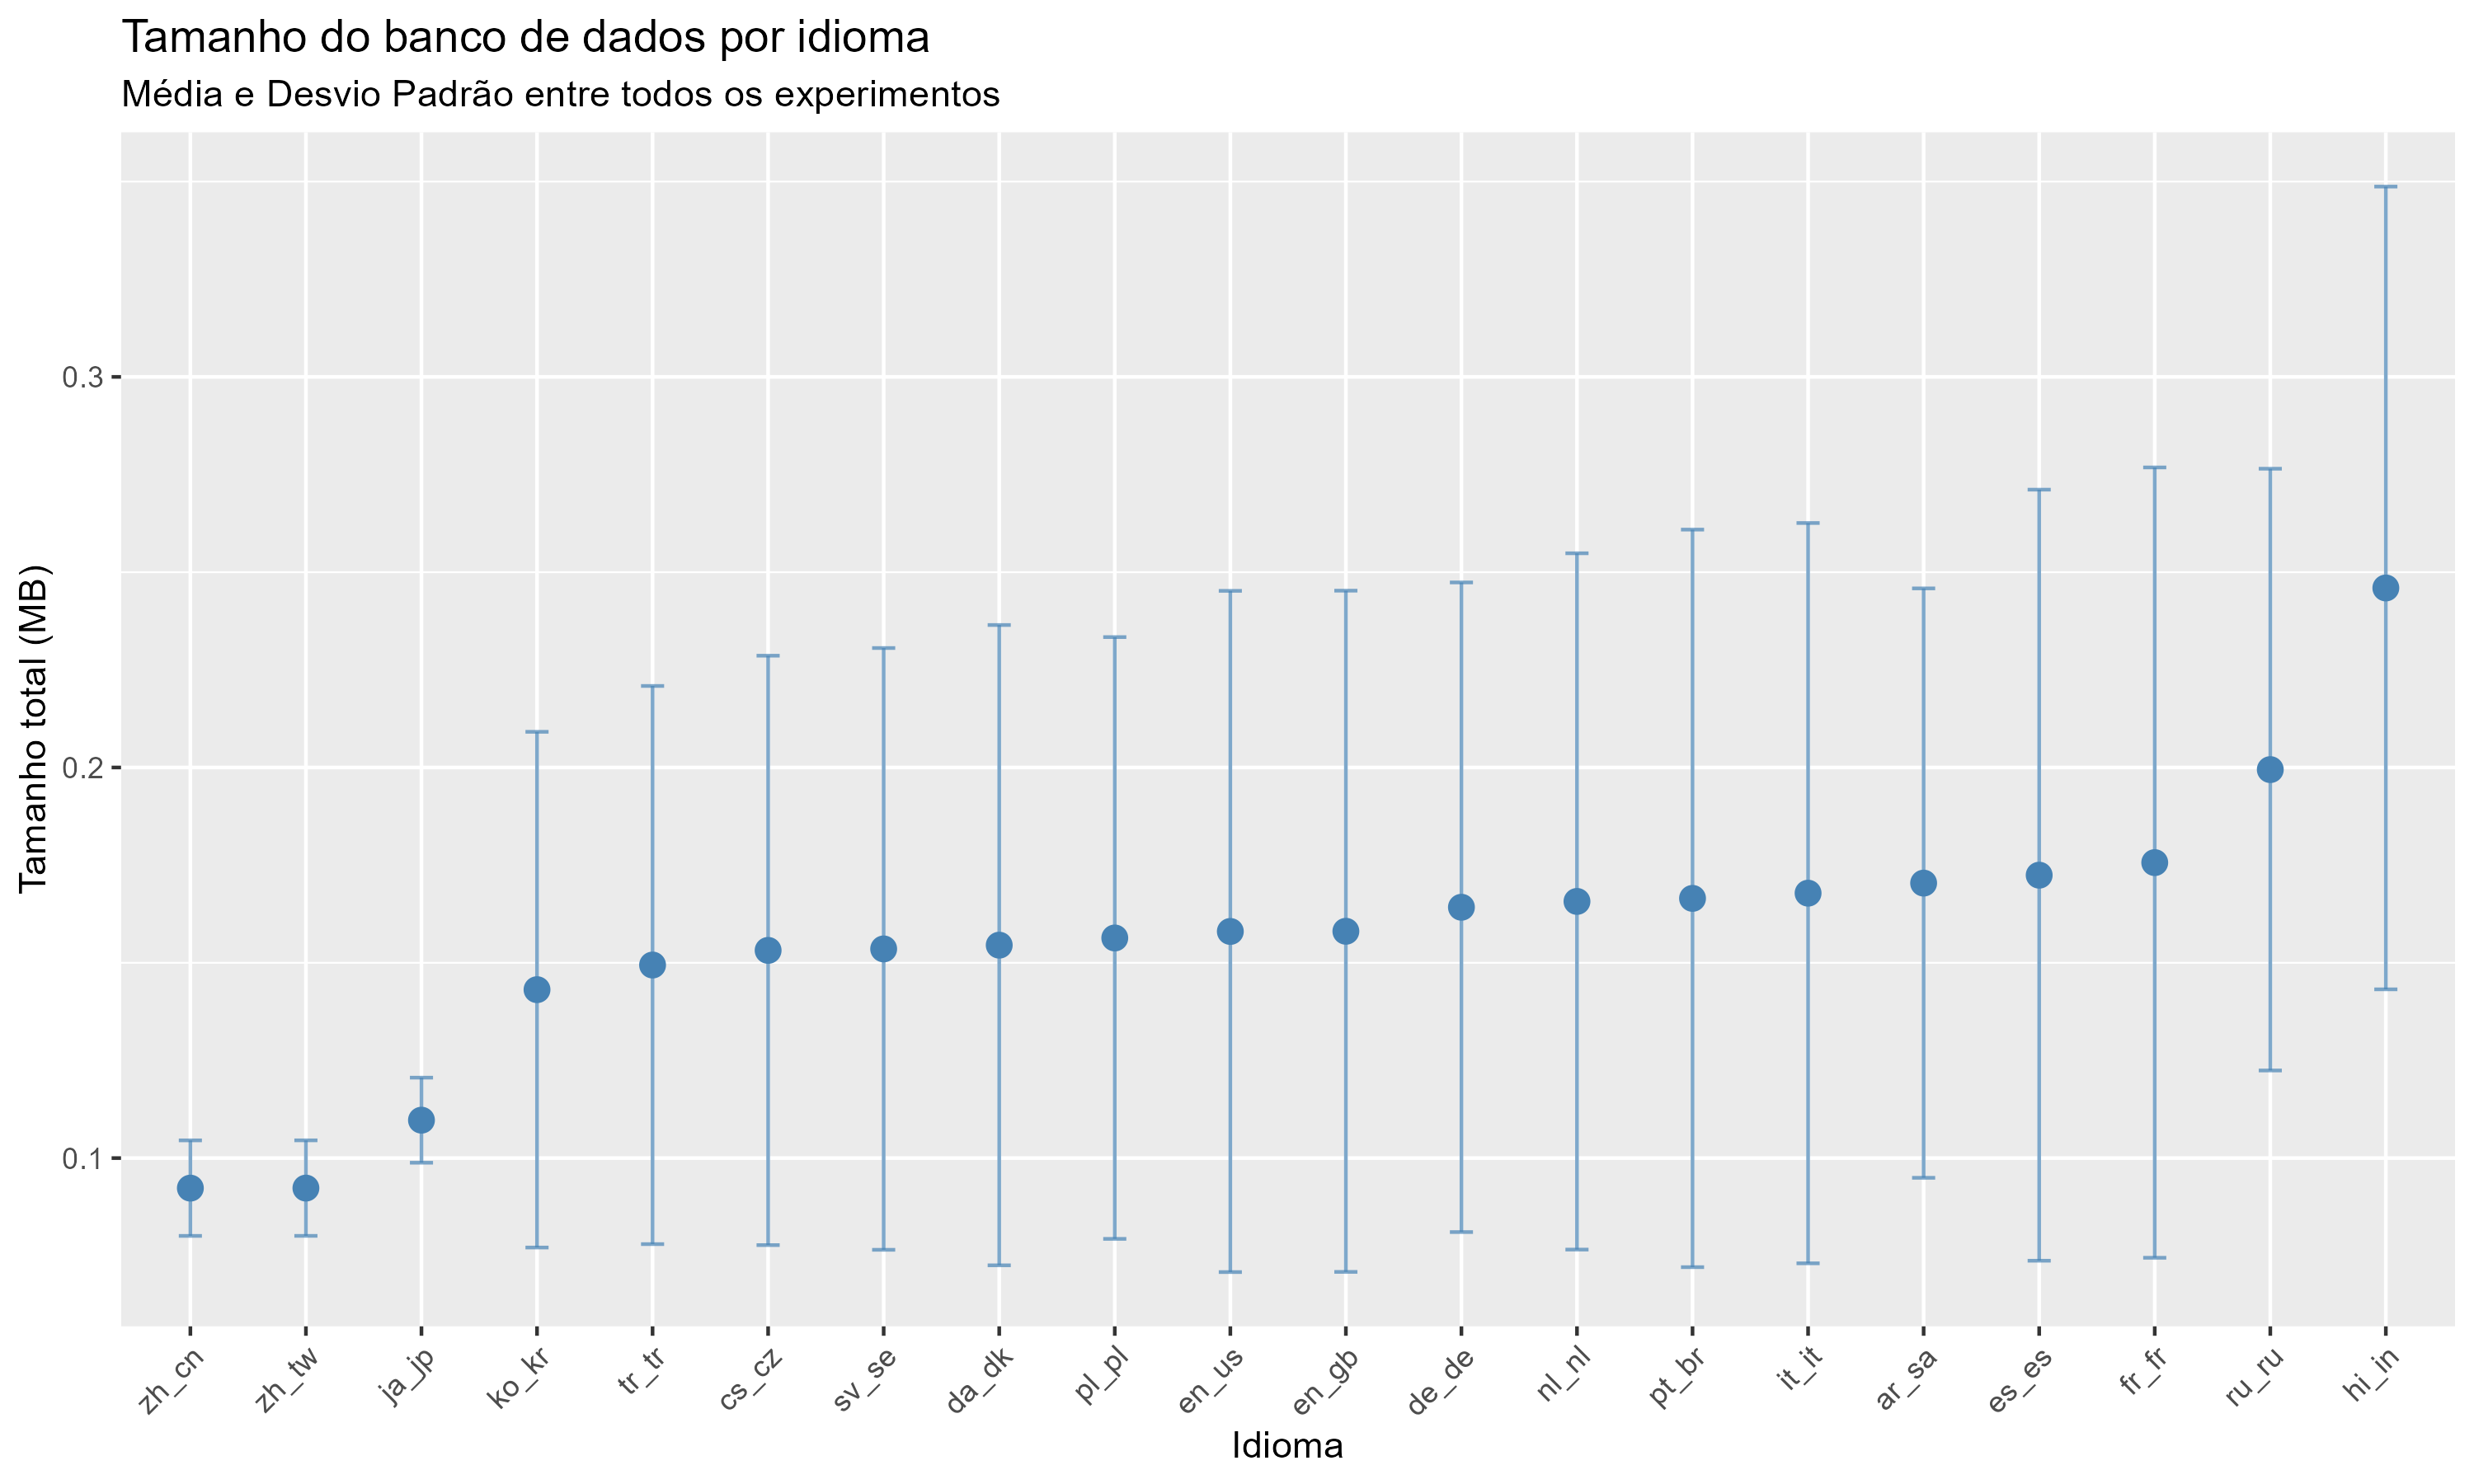
\includegraphics[width=0.8\linewidth]{../../src/results/graphs/g3_storage_size_all.png}
    \caption{Tamanho total de armazenamento do índice vetorial e metadados por idioma.}
    \label{fig:storage_size}
\end{figure}

\subsection{Tempo de Embedding por Idioma}
O custo computacional da etapa de \textit{encoding} com o modelo \texttt{intfloat/multilingual-e5-large} foi rastreado cronometricamente. A Figura \ref{fig:embedding_time_lang} demonstra o tempo médio de geração de embeddings por idioma, enquanto a Figura \ref{fig:embedding_time_chars} correlaciona diretamente esse tempo de processamento ao volume de caracteres (complexidade do arquivo).

\begin{figure}[htbp]
    \centering
    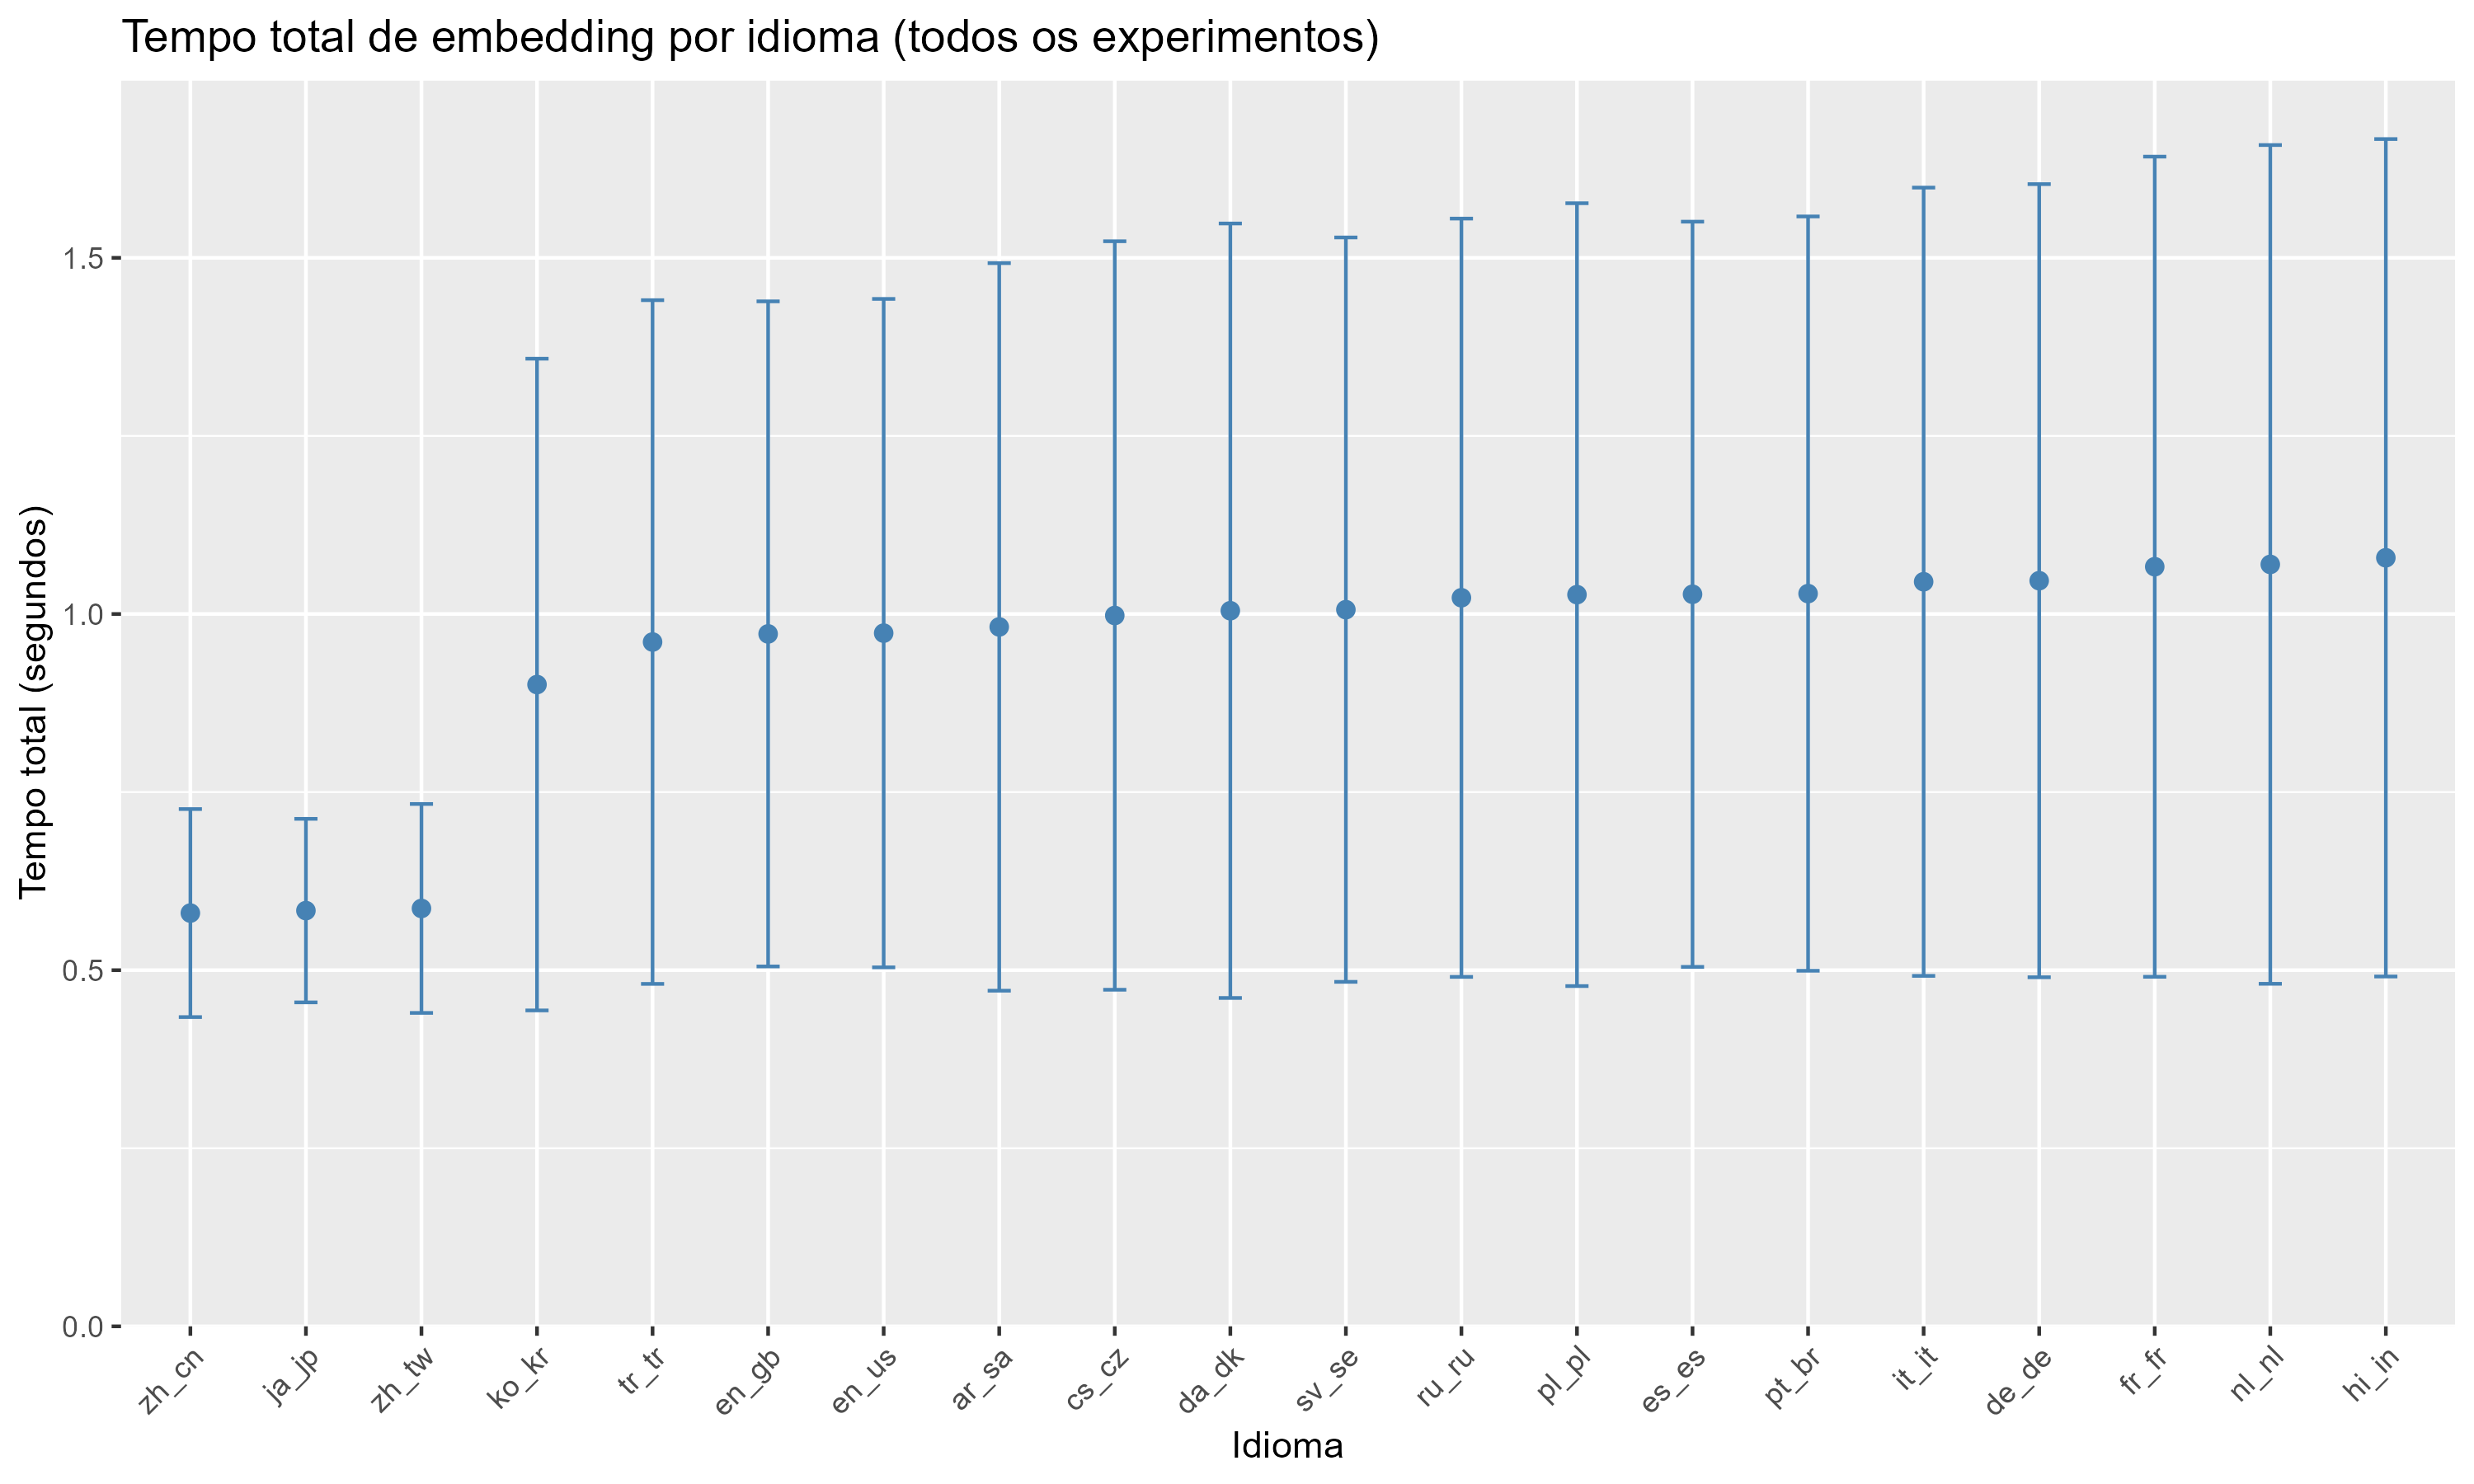
\includegraphics[width=0.8\linewidth]{../../src/results/graphs/g4_embedding_time_by_language_all.png}
    \caption{Tempo absoluto de geração de embeddings agrupado por idioma testado.}
    \label{fig:embedding_time_lang}
\end{figure}

\begin{figure}[htbp]
    \centering
    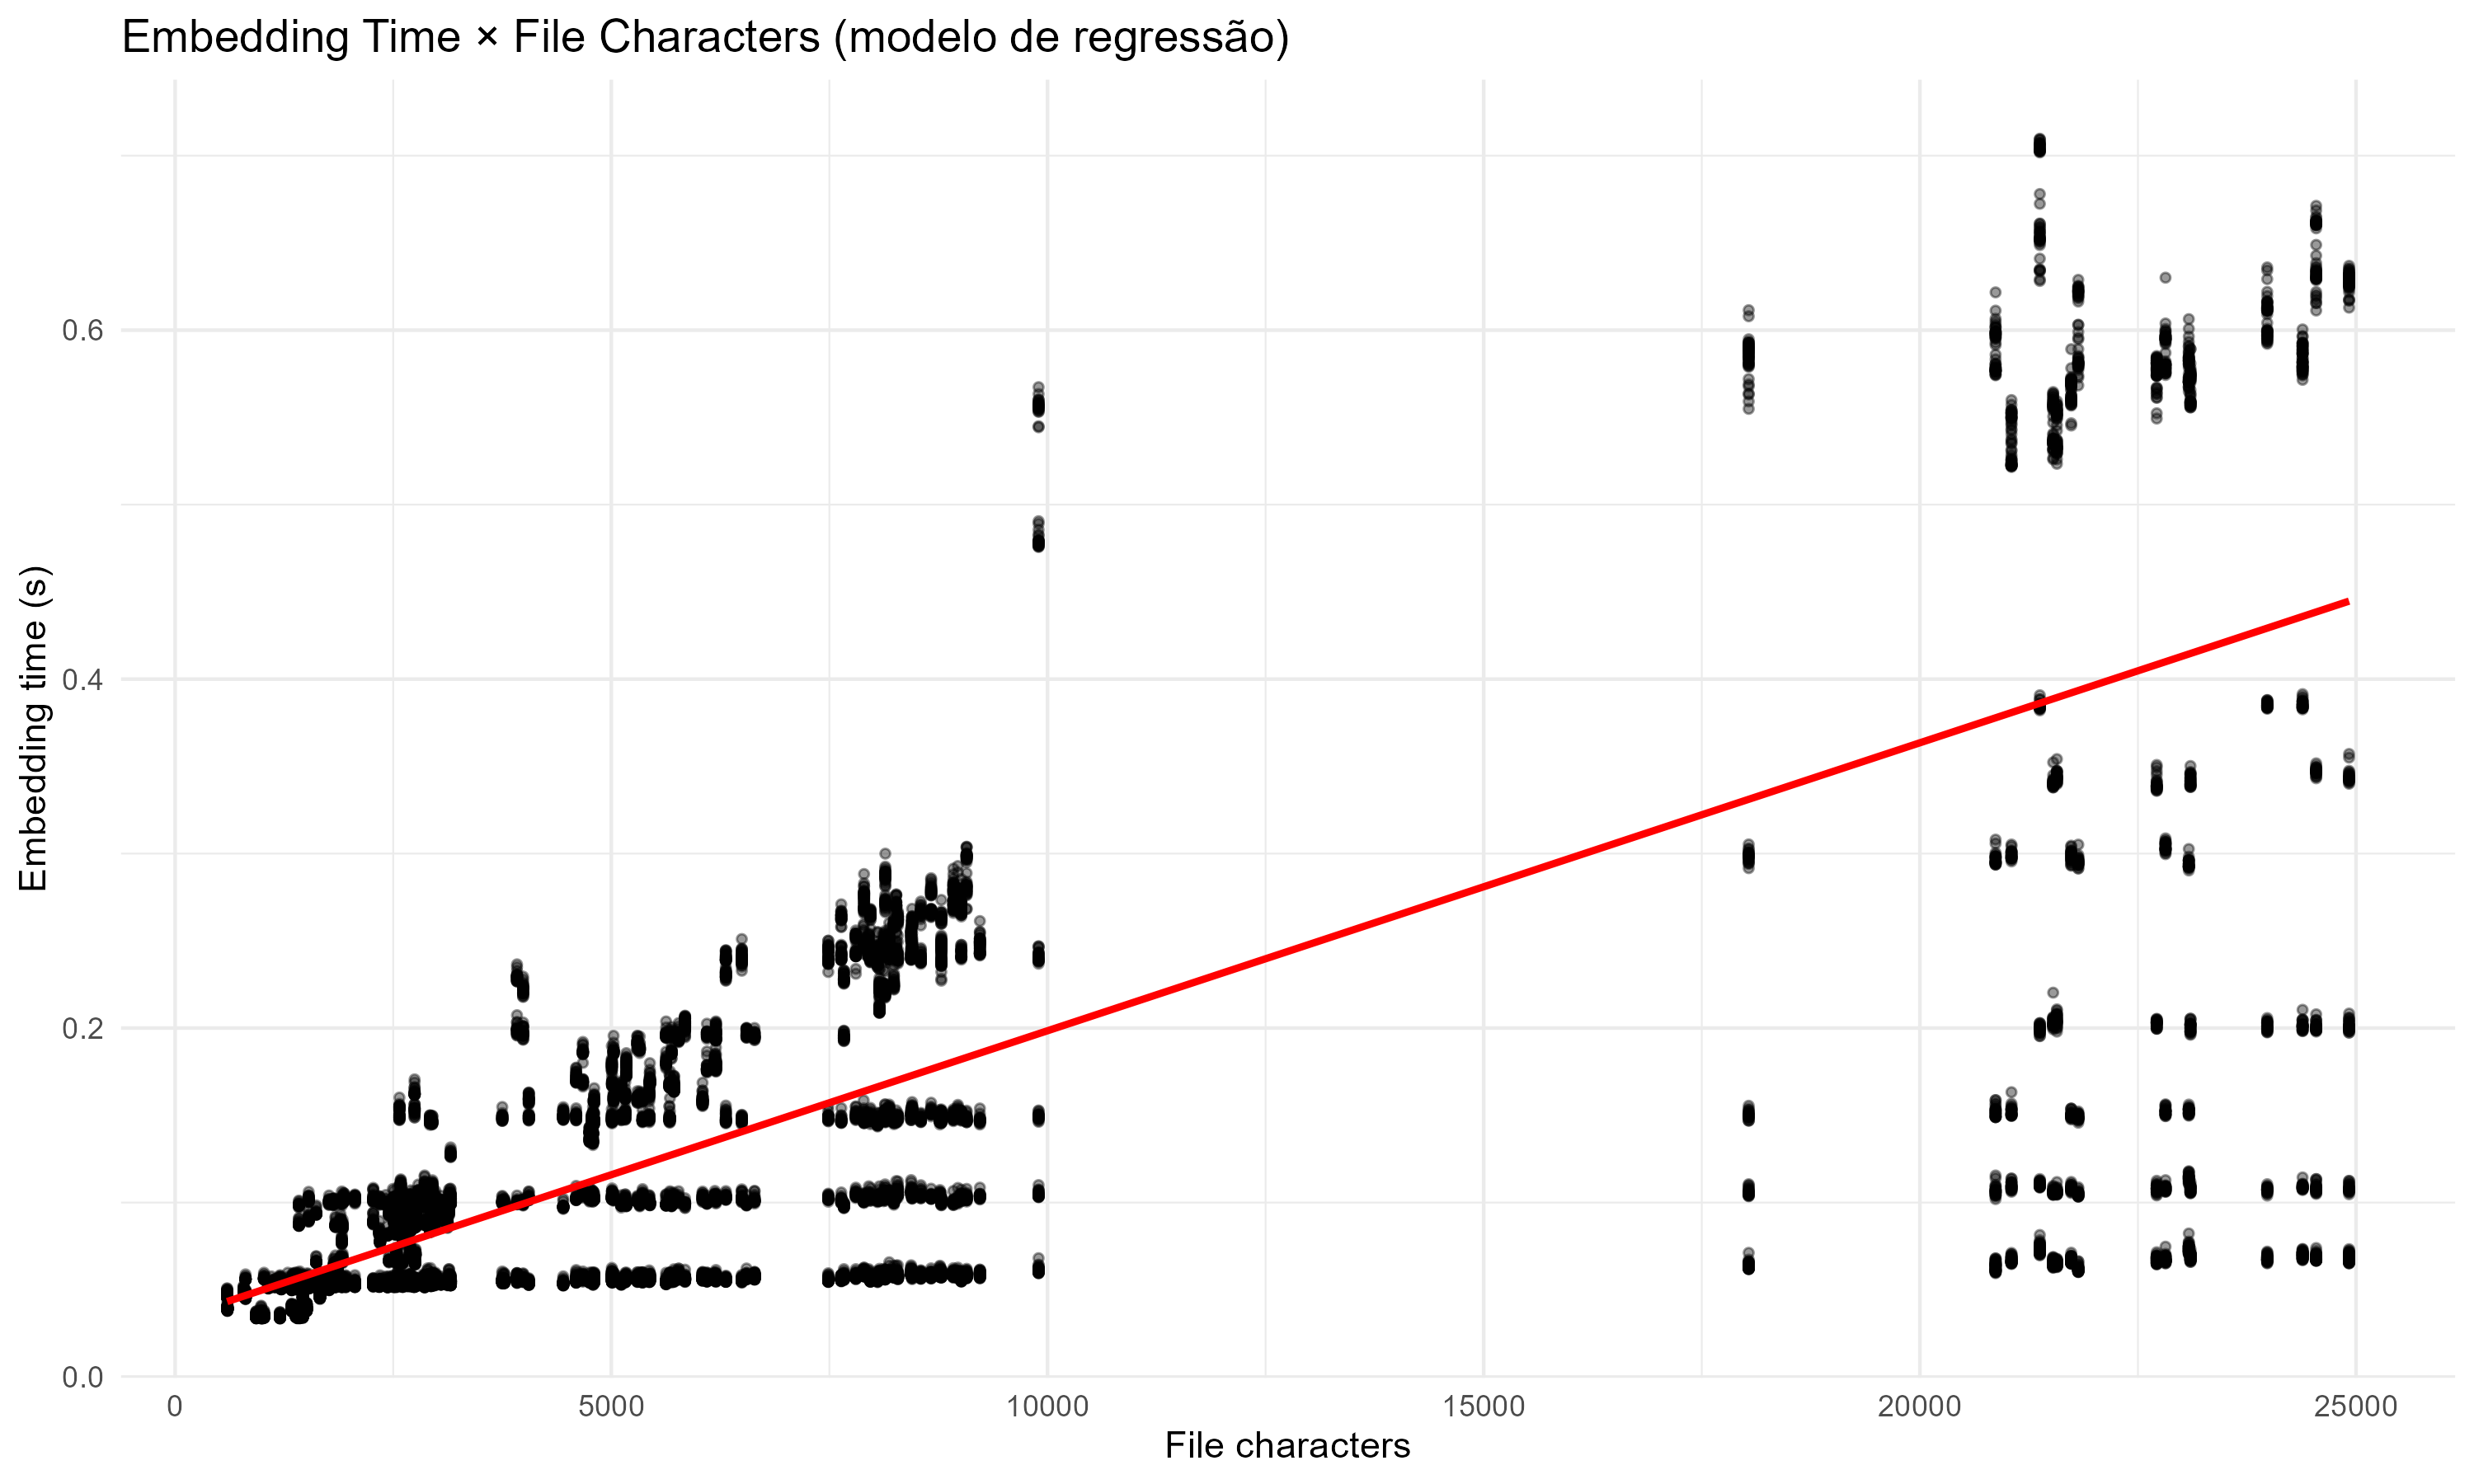
\includegraphics[width=0.8\linewidth]{../../src/results/graphs/embedding_time_vs_file_chars_model.png}
    \caption{Correlação entre o tempo de geração de embeddings e a quantidade de caracteres do documento.}
    \label{fig:embedding_time_chars}
\end{figure}

\subsection{Tamanho do Fragmento (Chunk Size) vs. Armazenamento Total}
A escolha do \texttt{chunk\_size} controla o equilíbrio entre contexto semântico e granularidade. A Figura \ref{fig:chars_vs_storage} explicita o impacto dessa parametrização no armazenamento total: fragmentos menores geram um número maior de vetores densos e sobrecargas de metadados, inflando o tamanho final do índice independentemente do idioma.

\begin{figure}[htbp]
    \centering
    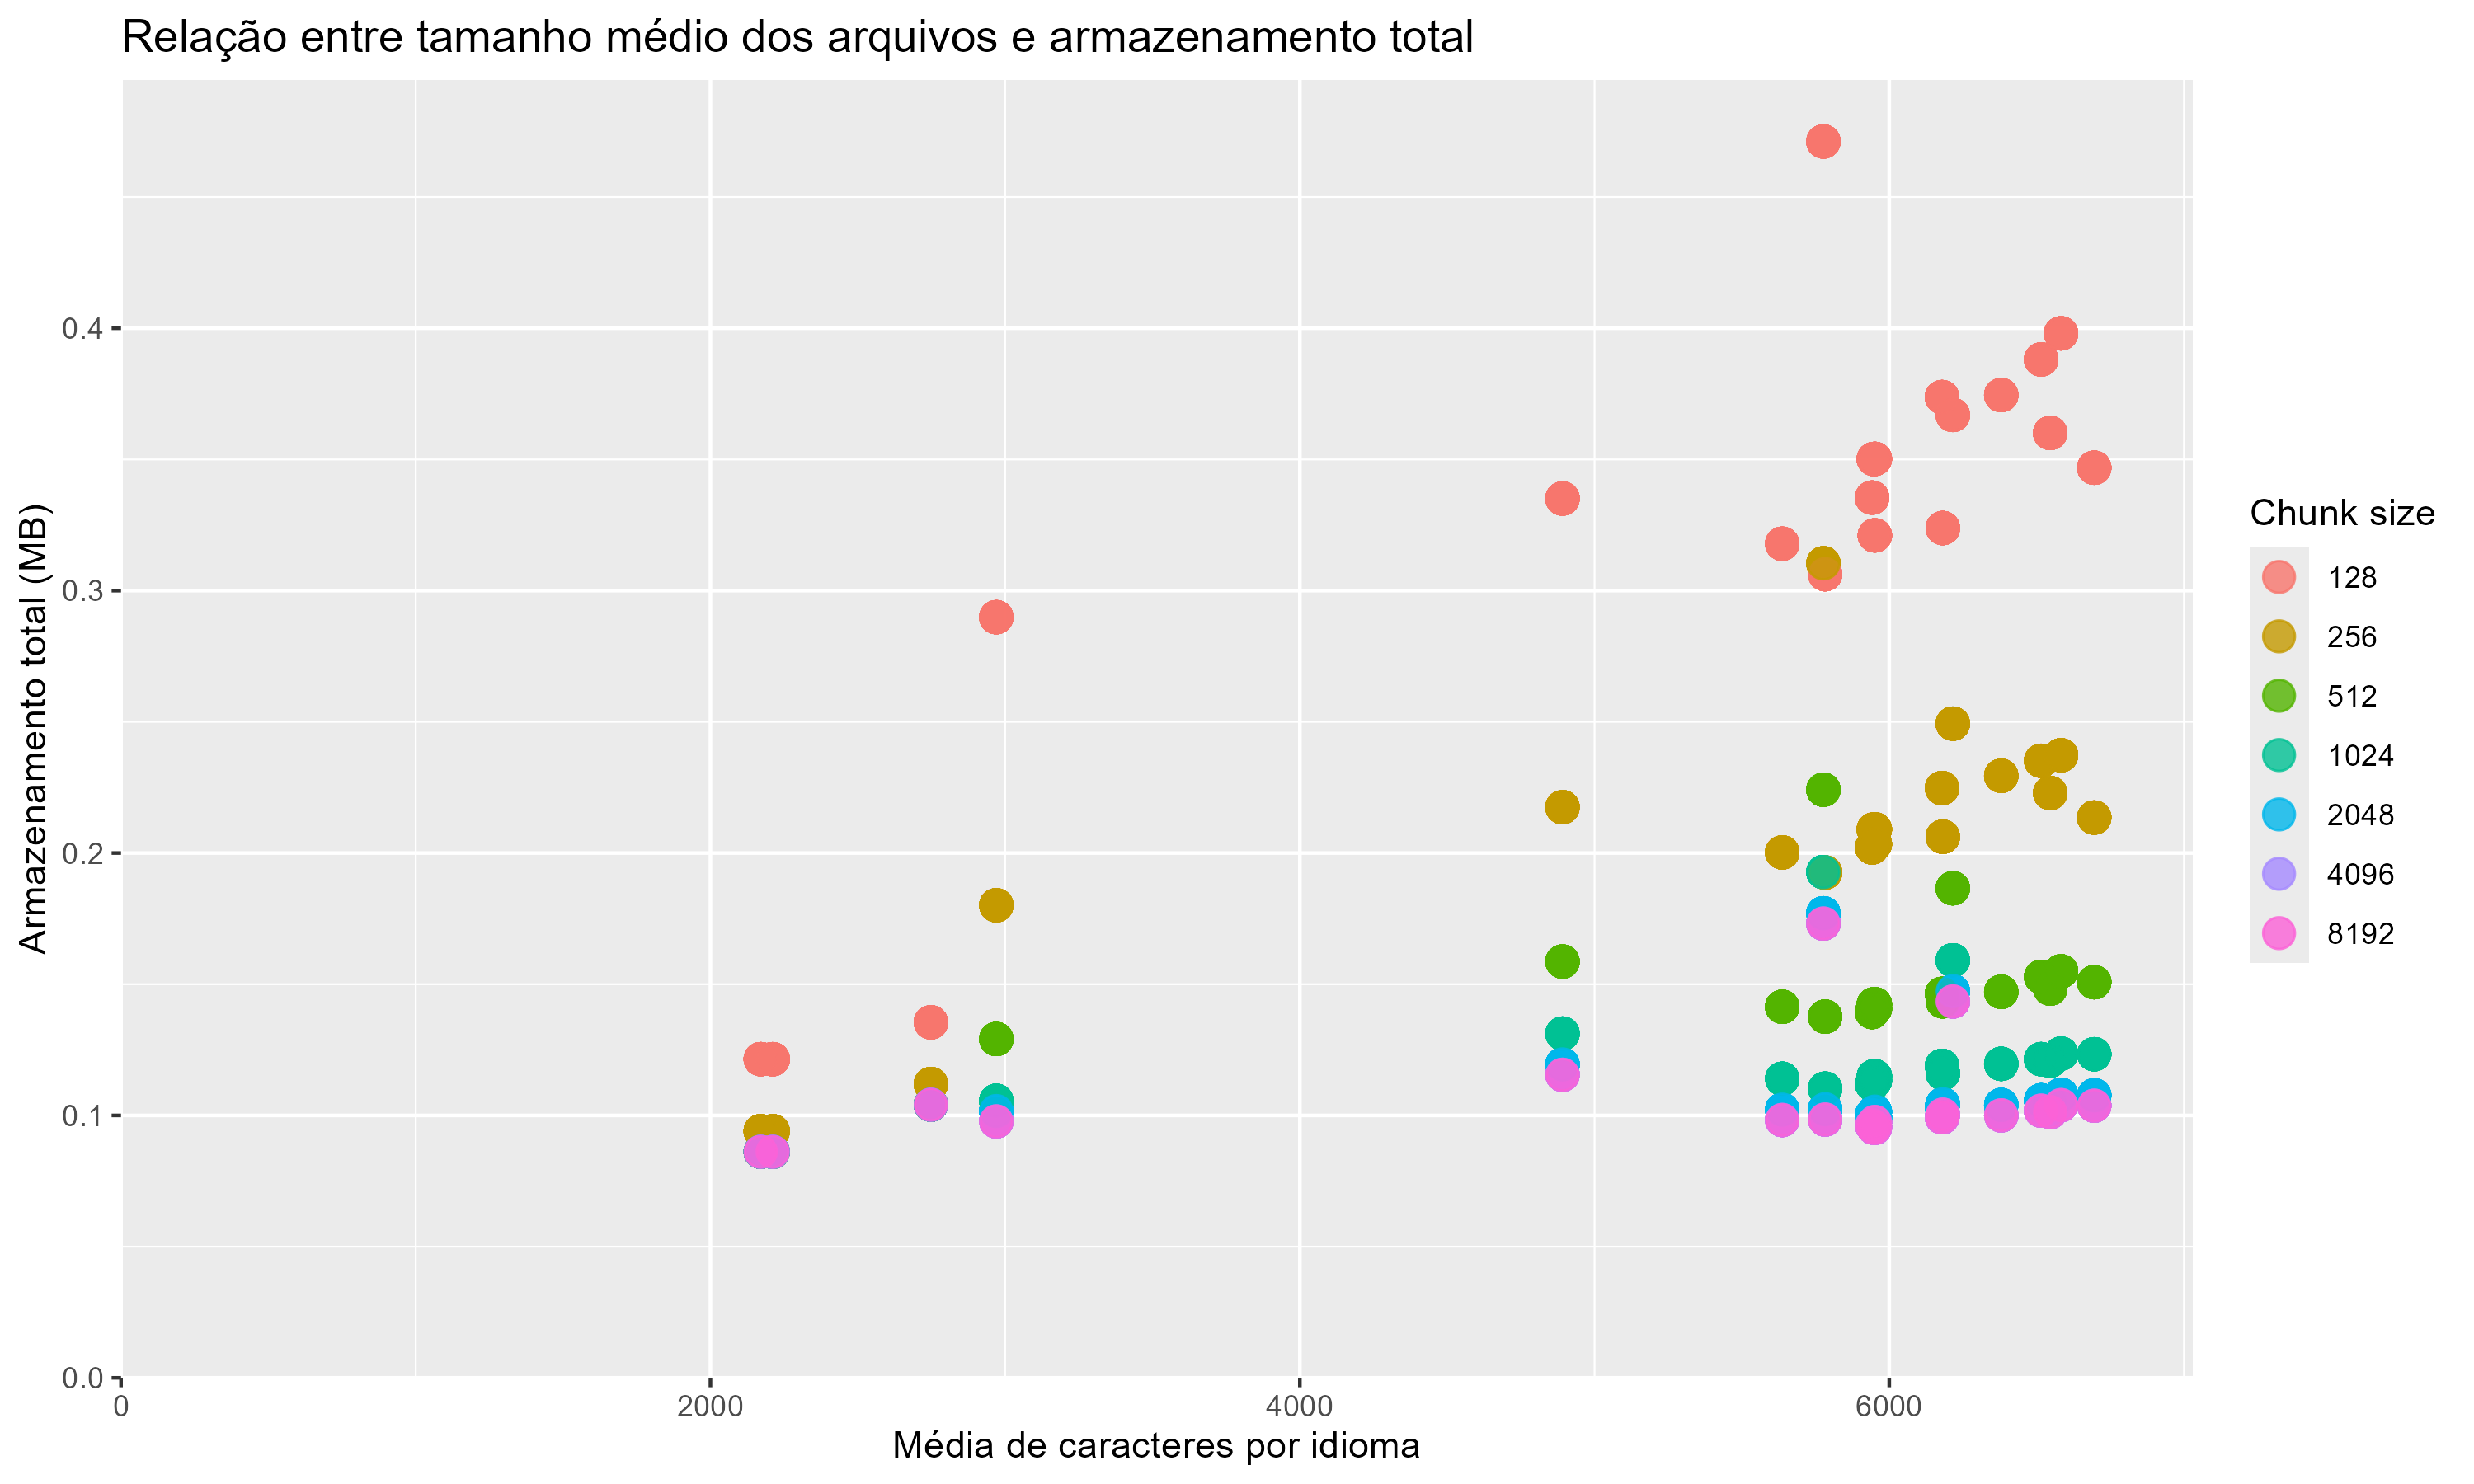
\includegraphics[width=0.8\linewidth]{../../src/results/graphs/g5_avg_chars_vs_storage.png}
    \caption{Relação entre a média de caracteres do \textit{chunk} e o armazenamento total exigido pelo índice.}
    \label{fig:chars_vs_storage}
\end{figure}

\subsection{Avaliação das Consultas (Queries)}
Para a validação do pipeline de recuperação, foram elaboradas 20 perguntas distintas. De forma análoga à abordagem adotada para os arquivos da base de conhecimento, essas consultas foram inicialmente construídas em inglês e, posteriormente, traduzidas para os demais idiomas-alvo com o auxílio do LLM \textit{GPT-5.1}. Como resultado desse mapeamento combinatório, o volume de dados experimentais foi expandido significativamente: a matriz que anteriormente totalizava 39.200 linhas deu origem a um novo arquivo \textit{CSV} consolidado com 784.000 linhas.

A partir desse conjunto, a etapa de recuperação baseou-se nas 20 consultas determinísticas avaliadas com $Top\_K = 6$, validadas diretamente contra um \textit{Gold Standard}. O desempenho semântico variou significativamente conforme o idioma alvo. A Figura \ref{fig:worst_rank} destaca os idiomas que apresentaram as piores posições no ranqueamento do documento correto, enquanto a Figura \ref{fig:best_rank} ilustra os idiomas com as buscas mais precisas. A latência de recuperação da árvore FAISS também sofreu variações representadas na Figura \ref{fig:retrieval_time}. Por fim, a Figura \ref{fig:gold_false} sumariza a porcentagem de falhas (casos em que o documento correto não foi retornado no Top-K) por idioma ao longo de todos os experimentos.

\begin{figure}[htbp]
    \centering
    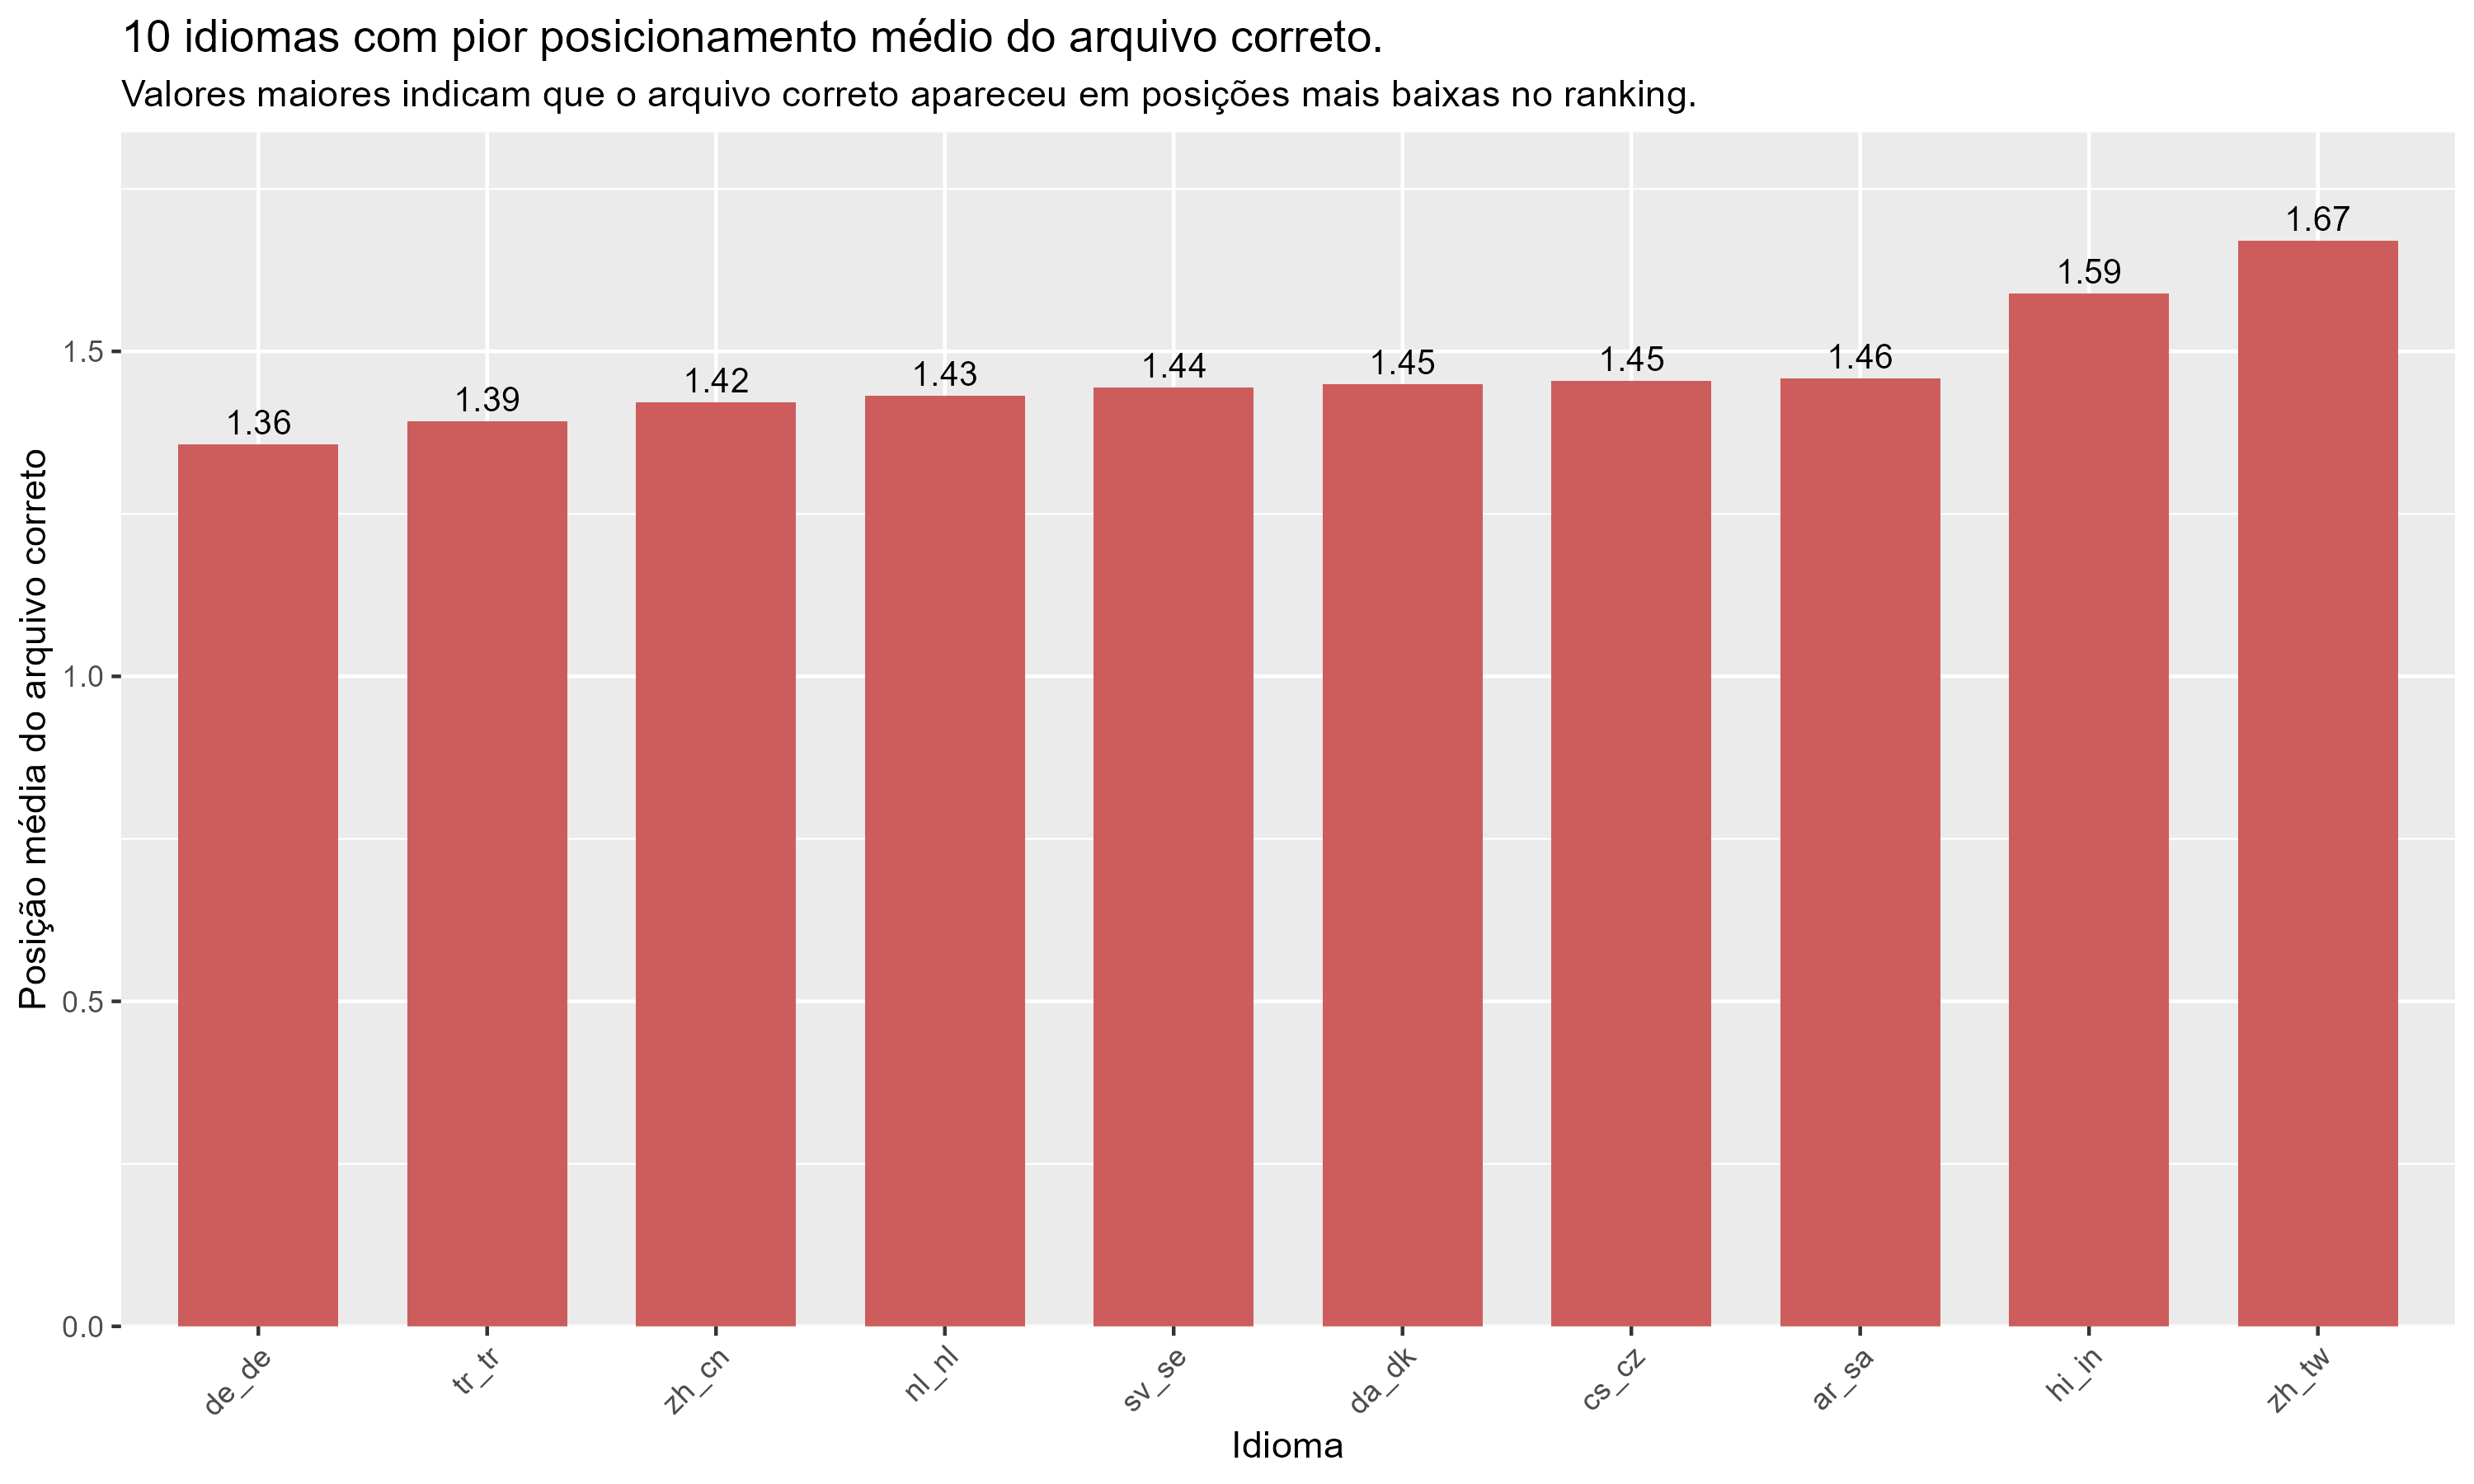
\includegraphics[width=0.8\linewidth]{../../src/results/graphs/g6_worst_gold_rank_languages_all_experiments.png}
    \caption{Idiomas com as piores posições médias no ranking de recuperação do documento alvo (\textit{Gold Rank}).}
    \label{fig:worst_rank}
\end{figure}

\begin{figure}[htbp]
    \centering
    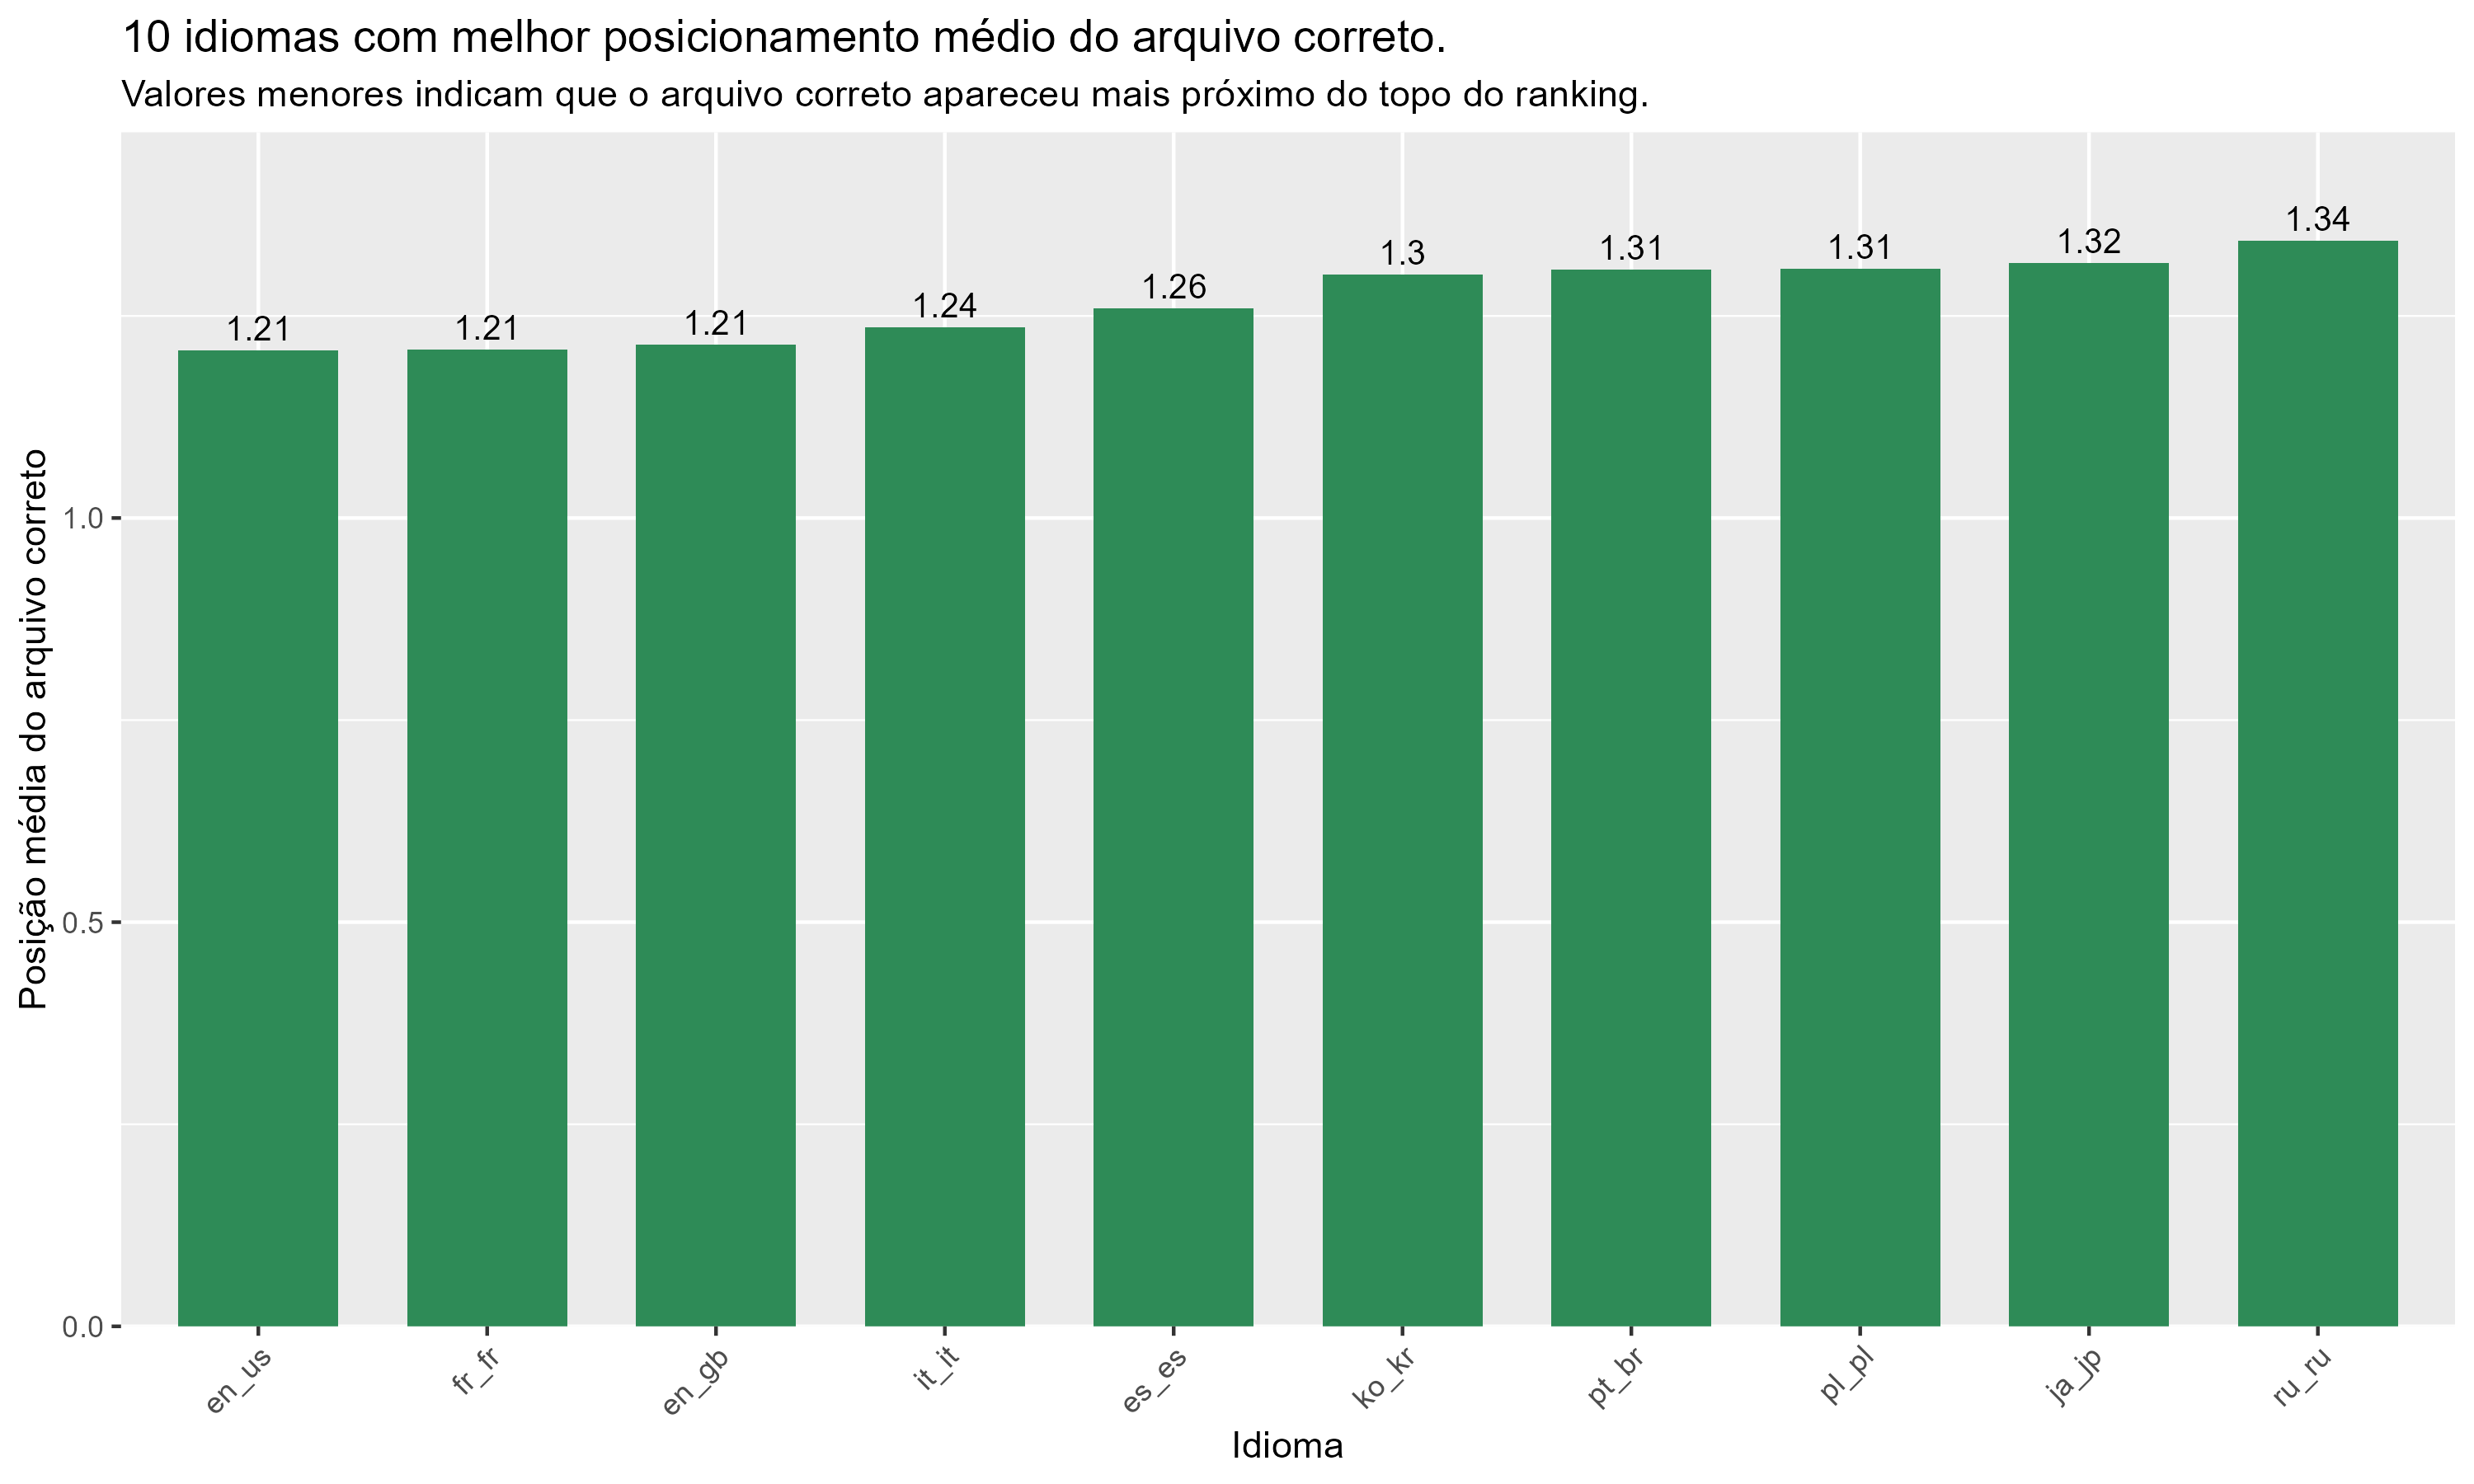
\includegraphics[width=0.8\linewidth]{../../src/results/graphs/g7_best_gold_rank_languages_all_experiments.png}
    \caption{Idiomas com as melhores posições médias no ranking de recuperação do documento alvo (\textit{Gold Rank}).}
    \label{fig:best_rank}
\end{figure}

\begin{figure}[htbp]
    \centering
    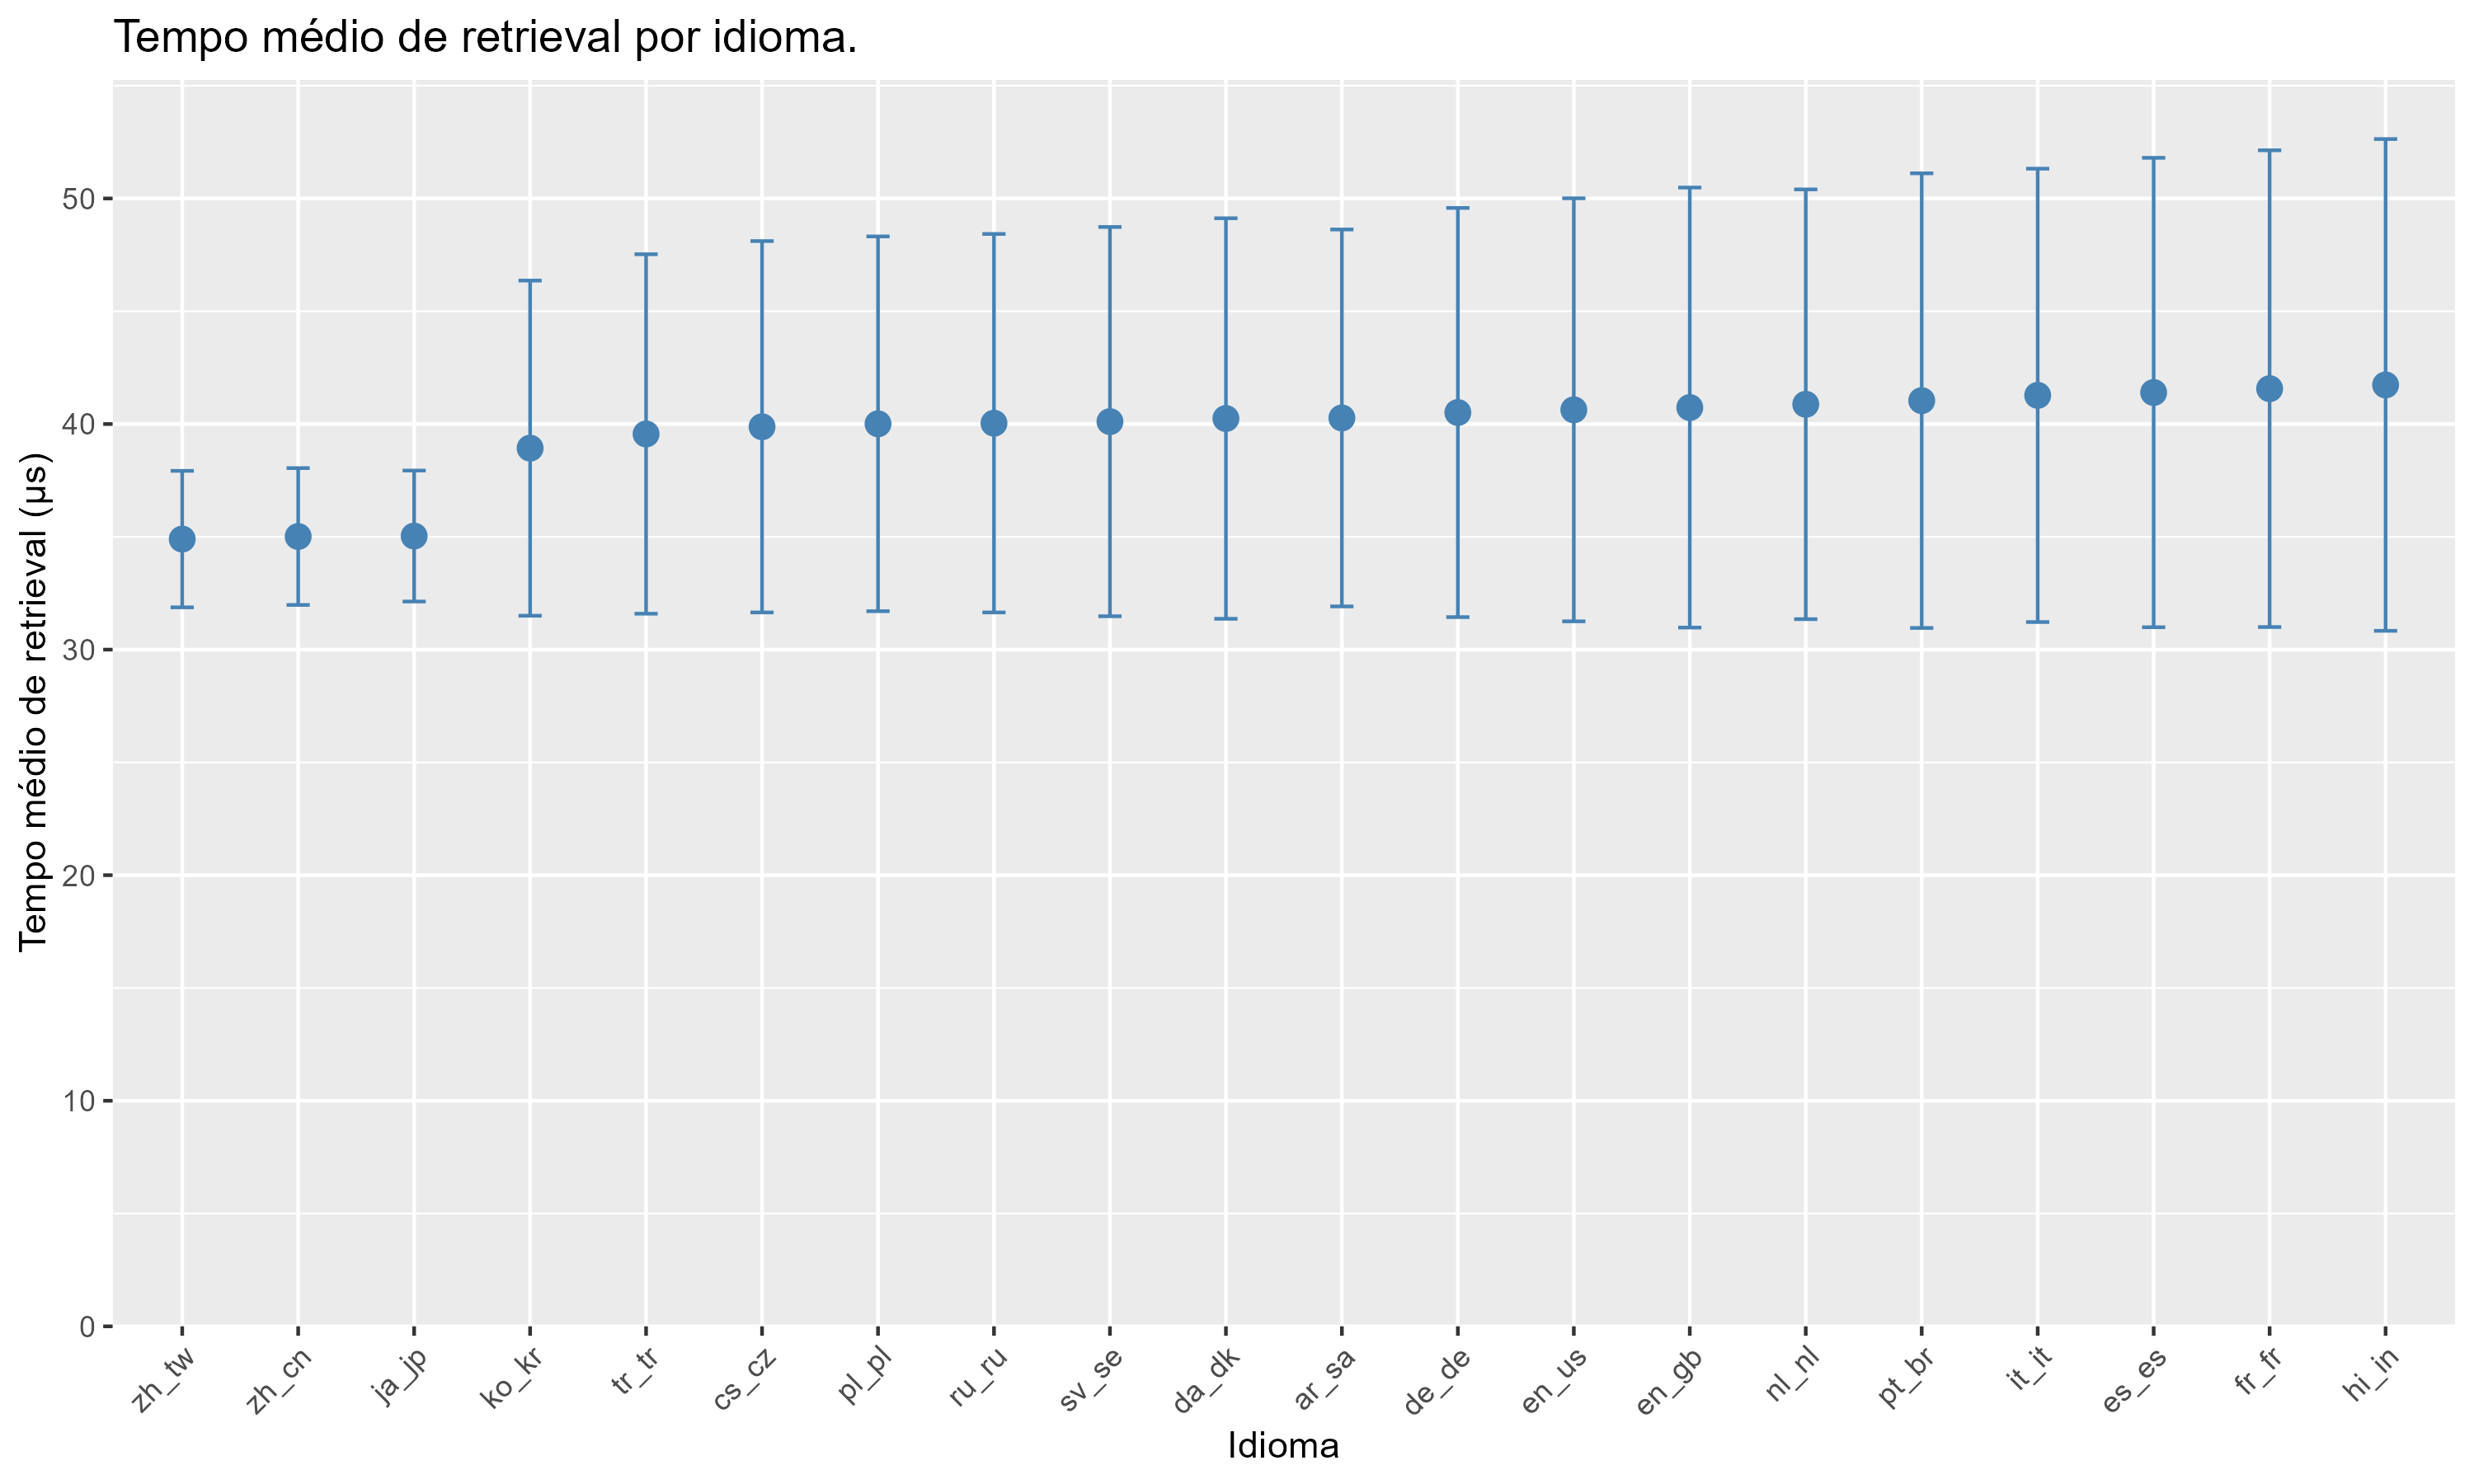
\includegraphics[width=0.8\linewidth]{../../src/results/graphs/g8_mean_retrieval_time_by_language_all_experiments.png}
    \caption{Tempo médio de recuperação (\textit{retrieval time}) em segundos por idioma.}
    \label{fig:retrieval_time}
\end{figure}

\begin{figure}[htbp]
    \centering
    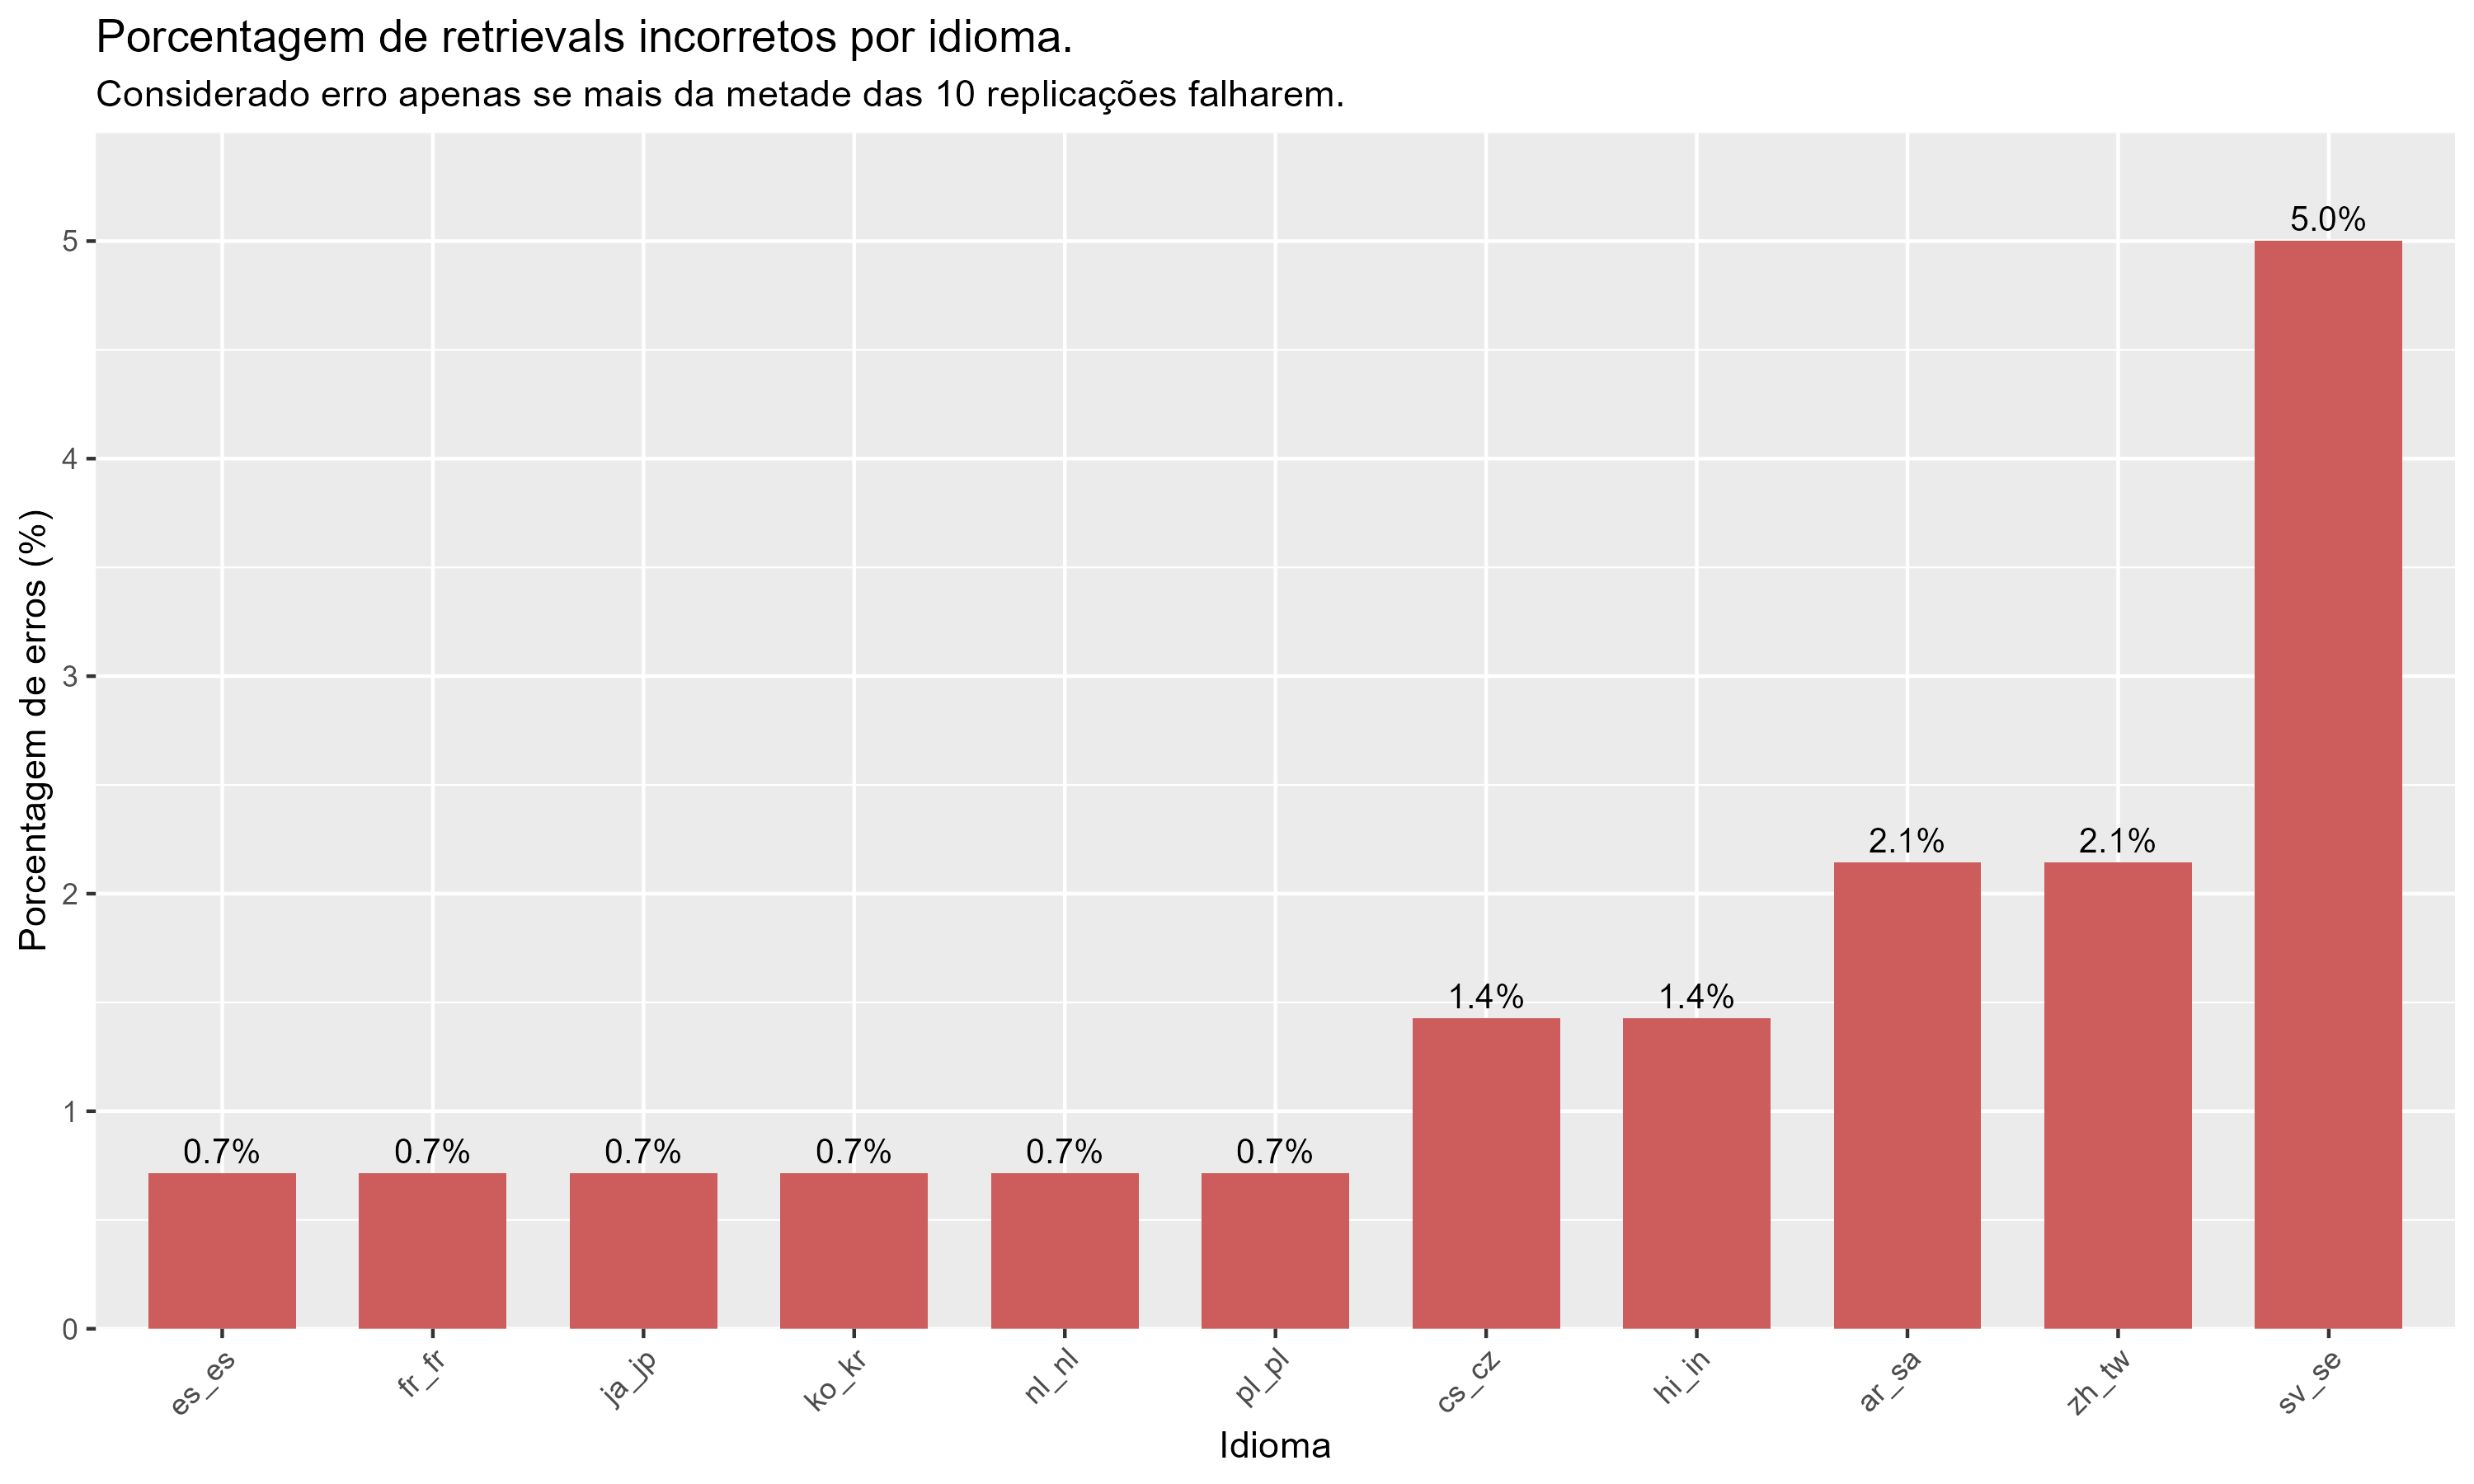
\includegraphics[width=0.8\linewidth]{../../src/results/graphs/g9_gold_false_percentage_by_language_all_experiments.png}
    \caption{Percentual de falhas absolutas (\textit{Gold False}) na recuperação por idioma ao longo dos testes.}
    \label{fig:gold_false}
\end{figure}

\section{Discussão}
Os resultados obtidos evidenciam que a homogeneização da busca semântica em múltiplos idiomas constitui um desafio complexo, comprovando que a língua afeta diretamente a qualidade e a eficiência de um sistema RAG (\textit{Retrieval-Augmented Generation}). Observou-se que idiomas mais verbosos tendem a consumir maior espaço de armazenamento no índice e a apresentar maior latência durante a etapa de \textit{retrieval}. Em contrapartida, idiomas mais sucintos demandam menos recursos de disco e, consequentemente, garantem buscas mais rápidas.

Apesar das variações estruturais entre as diferentes línguas, o inglês e o francês demonstraram o melhor desempenho geral em termos de eficácia e tempo de resposta. Este comportamento pode ser explicado pelo viés de treino do modelo base, que muito provavelmente foi exposto a um volume maior de dados nessas duas línguas durante o treinamento, o que pode ter otimizado a sua precisão semântica e a granularidade do contexto nesses idiomas. No extremo oposto, idiomas como \texttt{sv\_se} e \texttt{zh\_tw} registaram as piores métricas de \textit{retrieval}, cenário no qual o \textit{pipeline} falhou repetidamente em localizar e recuperar o ficheiro correto.

\section{Declaração de Uso de Inteligência Artificial}
Em conformidade com as diretrizes contemporâneas de transparência acadêmica e boas práticas de pesquisa corporativa, declara-se que ferramentas de Inteligência Artificial Generativa (Modelos de Linguagem de Grande Escala) foram utilizadas como assistentes de produtividade durante o desenvolvimento deste trabalho.

O uso dessas ferramentas concentrou-se majoritariamente nas fases de engenharia de software, atuando como suporte rápido para a pesquisa de soluções algorítmicas, depuração de erros e revisão de código-fonte (\textit{code review}) dos scripts responsáveis pela automação da coleta de métricas. Adicionalmente, as IAs foram empregadas para auxiliar na formatação tipográfica do documento em LaTeX, no refinamento estrutural do texto deste relatório técnico e na elaboração dos slides de apresentação para a defesa. Ressalta-se que a concepção arquitetural, o rigor metodológico, o raciocínio analítico e as conclusões extraídas dos dados são de autoria integral, exclusiva e sob responsabilidade estrita do autor.

\section{Conclusões}
A partir da análise dos dados experimentais, este estudo estabelece que:
\begin{enumerate}
    \item \textbf{O idioma determina a eficiência do \textit{pipeline}:} A verbosidade e a estrutura morfológica da língua afetam diretamente o consumo de armazenamento e a latência computacional. Idiomas mais verbosos exigem mais recursos de disco para o índice vetorial e aumentam os tempos de processamento tanto na geração de \textit{embeddings} quanto na etapa de \textit{retrieval}.
    \item \textbf{Existe um forte viés de desempenho focado no idioma inglês:} O inglês apresentou, de forma consistente, uma das melhores eficácias de recuperação e manteve um tempo de retrieval baixo. O modelo base demonstra um claro viés em relação aos seus dados de treino predominantes, resultando em falhas graves de recuperação para idiomas menos representados, como \texttt{sv\_se} e \texttt{zh\_tw}.
\end{enumerate}

\section{Trabalhos Futuros}
A infraestrutura parametrizada e a vasta matriz de resultados obtida através do DoE pavimentam o caminho para investigações mais profundas:
\begin{itemize}
    \item \textbf{Mitigação do Viés Linguístico:} Investigar técnicas de \textit{fine-tuning} em modelos de \textit{embedding} ou o uso de técnicas de alinhamento semântico para otimizar especificamente o ranqueamento dos idiomas que apresentaram as piores métricas de recuperação (como o Sueco e o Chinês Tradicional).
    \item \textbf{Avaliação de Modelos Alternativos:} Testar outros modelos de \textit{embeddings} multilingues para avaliar se o viés observado é específico do modelo atual ou uma tendência geral.
\end{itemize}

\begin{thebibliography}{9}
\bibitem{e5} Intfloat, \emph{multilingual-e5-large}.
\bibitem{qwen} Qwen Team, \emph{Qwen2.5 7B}.
\end{thebibliography}

\end{document}